\documentclass[cjk]{beamer}
\mode<presentation>{
  %\usetheme{Warsaw}
  \usetheme{CambridgeUS}
  \usecolortheme{beaver}
  \setbeamercovered{transparent}
}
\usepackage{titlesec} %设置标题
\usepackage{titletoc}
\usepackage{extarrows}
\usepackage{verbatim,color,xcolor}
\usepackage{pgf}
\usepackage{tikz}
\usetikzlibrary{calc}
\usetikzlibrary{arrows,snakes,backgrounds,shapes,patterns}
\usetikzlibrary{matrix,fit,positioning,decorations.pathmorphing}
%% \usepackage{classicthesis}
\usepackage{CJK}
\usepackage{mathdots}

\usepackage{listings}
\lstset{
keywordstyle=\color{blue!70},
frame=single,
basicstyle=\ttfamily\small,
commentstyle=\small\color{red},
breakindent=0pt,
rulesepcolor=\color{red!20!green!20!blue!20},
rulecolor=\color{black},
tabsize=4,
numbersep=5pt,
breaklines=true,
%% backgroundcolor=\color{red!10},
showspaces=false,
showtabs=false,
extendedchars=false,
escapeinside=``,
frame=no,
}

\input{definecolor.tex}
\def\blue{\textcolor{blue}}
\def\red{\textcolor{red}}
\def\purple{\textcolor{purple}}
\def\ds{\displaystyle}
\def\cd{\cdots}
\def\dd{\ddots}
\def\vd{\vdots}
\def\id{\iddots}

\def\A{\boldsymbol{A}}
\def\B{\boldsymbol{B}}
\def\C{\boldsymbol{C}}
\def\E{\boldsymbol{E}}
\def\F{\boldsymbol{F}}
\def\R{\mathbb R}

\def\nn{{\boldsymbol{n}}}
\def\xx{{\boldsymbol{x}}}
\def\bb{{\boldsymbol{b}}}
\def\tf{\ttfamily}
\def\zero{\boldsymbol{0}}
\def\II{\boldsymbol{I}}
\def\LLambda{\boldsymbol{\Lambda}}



\begin{document}
\begin{CJK}{UTF8}{gkai} 
  \CJKtilde
  \renewcommand{\proofname}{\vspace{0.2cm}\textbf{证明: \ }}
  \newcommand{\jiename}{\vspace{0.2cm}\textbf{解: \ }}
  
  \renewcommand{\figurename}{图}  
  \input{title.tex}
  
  
  \begin{frame}
    \titlepage
  \end{frame}

  \begin{frame}
    \frametitle{目录}
    \tableofcontents[currentsection]
  \end{frame}

  \AtBeginSection[]{
    \begin{frame}[allowframebreaks]
      \tableofcontents[currentsection]%,hideallsubsections]
    \end{frame}
  }
  \AtBeginSubsection[]{
    \begin{frame}[shrink]
      \tableofcontents[sectionstyle=show/shaded,subsectionstyle=show/shaded/hide]
    \end{frame}
  }


  \section{矩阵的定义}
\begin{dingyi}
  由$m\times n$个数$a_{ij}(i=1,2,\cd,m; \ j = 1, 2, \cd, n)$排成的$m$行$n$列的数表
  $$
  \begin{array}{cccc}
    a_{11} & a_{12} & \cd & a_{1n}\\
    a_{21} & a_{22} & \cd & a_{2n}\\
    \vd    & \vd   &     & \vd \\
    a_{m1} & a_{m2} & \cd & a_{mn}\\
  \end{array}
  $$
  称为$m$行$n$列矩阵,简称$m \times n$矩阵,记作
  $$
  {\A} = \left(
  \begin{array}{cccc}
    a_{11} & a_{12} & \cd & a_{1n}\\
    a_{21} & a_{22} & \cd & a_{2n}\\
    \vd    & \vd   &     & \vd \\
    a_{m1} & a_{m2} & \cd & a_{mn}\\
  \end{array}
  \right),
  $$
  这$m \times n$个数称为$\A$的元素
  ,数$a_{ij}$位于矩阵$\A$的第$i$行第$j$列,
  称为矩阵的$(i,j)$元。 可简记为\red{$(a_{ij})$}、\red{$(a_{ij})_{m\times n}$}或\red{$\A_{m \times n}$}。
\end{dingyi}

\begin{zhu*}
  对矩阵的定义,需做以下几点说明:
  \begin{itemize}
  \item 
    元素是实数的矩阵称为\red{实矩阵},元素为复数的矩阵称为\red{复矩阵};
  \item
    行数与列数都等于$n$的矩阵称为$n$阶矩阵或$n$阶方阵。$n$阶矩阵$\A$也记作$\A_n$;
  \item
    只有一行的矩阵
    $$
    \A = \left(
    \begin{array}{cccc}
      a_1 & a_2 & \cd & a_n
    \end{array}
    \right )
    $$
    称为\red{行矩阵},又称\red{行向量},也记为
    $$
    \A = \left(
    \begin{array}{cccc}
      a_1, & a_2, & \cd, & a_n
    \end{array}
    \right );
    $$
  \item
    只有一列的矩阵
    $$
    \A = \left(
    \begin{array}{c}
      a_1 \\
      a_2 \\
      \vd \\
      a_n
    \end{array}
    \right )
    $$
    称为\red{列矩阵},又称\red{列向量}。
  \item 
    两行矩阵的行数相等、列数也相等时,称它们为\red{同型矩阵}。
  \item
    如果$\A=(a_{ij})$和$\mathbf{B}=(b_{ij})$是同型矩阵,
    且它们的对应元素相等,即
    $$
    a_{ij} = b_{ij}(i=1,2,\cd,m; \ j =1,2,\cd,n),
    $$
    则称矩阵$\A$与$\mathbf{B}$相等,记作
    $$
    \A = \mathbf{B}.
    $$
  \item
    元素都为0的矩阵称为\blue{零矩阵},记作{$\mathbf{O}$}。
    \red{注意不同型的零矩阵是不同的。}
  \end{itemize}
\end{zhu*}
\vspace{.1in} \noindent
接下来我们举几个例子介绍矩阵的应用。
\begin{li}
  某厂向三个商店发送四种产品的数量可列成矩阵
  \begin{figure}[htbp]
    \centering
    \begin{tikzpicture}
      \matrix (M) [matrix of math nodes]  { 
        \A = \\
      };
      \matrix(MM) [right=.5in of M, matrix of math nodes,nodes in empty cells,
        column sep=3ex,row sep=1.5ex,ampersand replacement=\&,left delimiter=(,right delimiter=)] {
        a_{11} \& a_{12} \& a_{13}  \\
        a_{21} \& a_{22} \& a_{23}  \\
        a_{31} \& a_{32} \& a_{33}  \\
        a_{41} \& a_{42} \& a_{43}  \\
      };
      \node[above=7pt  of MM-1-1, blue]  {商店1};
      \node[above=7pt  of MM-1-2, blue]  {商店2};
      \node[above=7pt  of MM-1-3, blue]  {商店3};
      \node[left =12pt  of MM-1-1, blue]  {产品1};
      \node[left =12pt  of MM-2-1, blue]  {产品2};
      \node[left =12pt  of MM-3-1, blue]  {产品3};
      \node[left =12pt  of MM-4-1, blue]  {产品4};
    \end{tikzpicture}
  \end{figure}
  
  其中$a_{ij}$为工厂向第$j$店发送第$i$种产品的数量。
  这四种产品的单价及单件重量也可列成矩阵
  \begin{figure}[htbp]
    \centering
    \begin{tikzpicture}
      \matrix (M) [matrix of math nodes]  { 
        \B = \\
      };
      \matrix(MM) [right=.5in of M, matrix of math nodes,nodes in empty cells,
        column sep=3ex,row sep=1.5ex,ampersand replacement=\&,left delimiter=(,right delimiter=)] {
        b_{11} \& b_{12}   \\
        b_{21} \& b_{22}   \\
        b_{31} \& b_{32}   \\
        b_{41} \& b_{42}   \\
      };
      \node[above=7pt  of MM-1-1, blue]  {单价};
      \node[above=7pt  of MM-1-2, blue]  {单件重量};
      \node[left =12pt  of MM-1-1, blue]  {产品1};
      \node[left =12pt  of MM-2-1, blue]  {产品2};
      \node[left =12pt  of MM-3-1, blue]  {产品3};
      \node[left =12pt  of MM-4-1, blue]  {产品4};
    \end{tikzpicture}
  \end{figure}
  
  其中$b_{i1}$为第$i$种产品的单价,$b_{i2}$为第$i$种产品的单件重量。
\end{li}

\begin{li}
  四个城市间的单向航线如图所示
  \tikzstyle{place}=[circle,draw=blue!50,fill=blue!20,thick]
  \begin{figure}[htbp]
    \begin{center}
      \begin{tikzpicture}[scale=1.2]
        \node(A) at (0,0) [place] {2};
        \node(B) at (2,0) [place] {3};
        \node(C) at (2,2) [place] {4};
        \node(D) at (0,2) [place] {1};            
        \draw[red,thick,<->] (A.north) -- (D.south);
        \draw[red,thick,->]  (C.south) -- (B.north);
        \draw[red,thick,->]  (D.south east) -- (B.north west);
        \draw[red,thick,<->] (D.east) -- (C.west);
        \draw[red,thick,<-]  (A.east) -- (B.west);
      \end{tikzpicture}
    \end{center}
  \end{figure}
  
  若令
  $$
  a_{ij} = \left\{
  \begin{array}{ll}
    1, & \mbox{从$i$市到$j$市有1条单向航线},\\[0.1in]
    0, & \mbox{从$i$市到$j$市没有单向航线},
  \end{array}
  \right.
  $$  
  则该航线图可用矩阵表示为
  \begin{figure}[htbp]
    \centering
    \begin{tikzpicture}[scale=0.5]
      \matrix (M) [matrix of math nodes]  { 
        \A = \\
      };
      \matrix(MM) [right=.5in of M, matrix of math nodes,nodes in empty cells,
        column sep=4ex,row sep=.05ex,ampersand replacement=\&,left delimiter=(,right delimiter=)] {
        0 \& 1 \& 1 \& 1\\
        1 \& 0 \& 0 \& 0\\
        0 \& 1 \& 0 \& 0\\
        1 \& 0 \& 1 \& 0\\
      };
      \node[above=2pt  of MM-1-1, blue]  {城市1};
      \node[above=2pt  of MM-1-2, blue]  {城市2};
      \node[above=2pt  of MM-1-3, blue]  {城市3};
      \node[above=2pt  of MM-1-4, blue]  {城市4};
      \node[left =12pt  of MM-1-1, blue]  {城市1};
      \node[left =12pt  of MM-2-1, blue]  {城市2};
      \node[left =12pt  of MM-3-1, blue]  {城市3};
      \node[left =12pt  of MM-4-1, blue]  {城市4};
    \end{tikzpicture}
  \end{figure}
\end{li}


\begin{li}
  设变量$x_1, x_2, \cd, x_n$与变量$y_1,y_2,\cd,y_m$满足:
  \begin{equation}\label{lt}
    \left\{
    \begin{array}{c}
      y_1  = a_{11} x_1 + a_{12} x_2 + \cd + a_{1n} x_n, \\[0.2cm]
      y_2  = a_{21} x_1 + a_{22} x_2 + \cd + a_{2n} x_n, \\[0.2cm]
      \vd \\[0.2cm]
      y_m  = a_{m1} x_1 + a_{m2} x_2 + \cd + a_{mn} x_n
    \end{array}
    \right.
  \end{equation}
  它表示一个从变量$x_1, x_2, \cd, x_n$到变量$y_1,y_2,\cd,y_m$的\red{线性变换}, 其系数$a_{ij}$构成矩阵$A=(a_{ij})_{m\times n}$。
\end{li}
\begin{itemize}
\item  给定了线性变换(\ref{lt}),其\red{系数矩阵}也就确定。 
\item   反之,若给出一个矩阵作为线性变换的系数矩阵,则线性变换也就确定。 
\item   从这个意义上讲,线性变换与矩阵之间存在一一对应的关系。
\end{itemize}      

(1)、线性变换
$$
\left\{
\begin{array}{c}
  y_1 = x_1, \\[0.2cm]
  y_2 = x_2, \\[0.2cm]
  \vd \\[0.2cm]
  y_n = x_n
\end{array}
\right.
$$
称为\red{恒等变换}, 它对应$n$阶方阵
$$
\mathbf{I} = \left(
\begin{array}{cccc}
  1    & 0    & \cd  & 0 \\
  0    & 1    & \cd  & 0 \\
  \vd  & \vd  &      & \vd \\
  0    & 0    & \cd  & 1
\end{array}
\right). 
$$ 
该方阵称为$n$阶\red{单位矩阵},简称\red{单位阵}。其$(i,j)$元为
$$
\delta_{ij} = \left \{
\begin{array}{ll}
  1, &i=j, \\
  0, &i\ne j.
\end{array}
\right.  
$$

(2)、线性变换
$$
\left\{
\begin{array}{c}
  y_1 = \lambda_1 x_1, \\[0.2cm]
  y_2 = \lambda_2 x_2, \\[0.2cm]
  \vd \\[0.2cm]
  y_n = \lambda_n x_n
\end{array}
\right.
$$  
对应于$n$阶方阵
$$
\A = \left(
\begin{array}{cccc}
  \lambda_1& 0    & \cd  & 0 \\
  0    & \lambda_2    & \cd  & 0 \\
  \vd  & \vd  &      & \vd \\
  0    & 0    & \cd  & \lambda_n
\end{array}
\right),
$$
这种方阵称为\red{对角矩阵},简称\red{对角阵},记作
$$
\A = \mathrm{diag}(\lambda_1,\lambda_2,\cd,\lambda_n).
$$

(3)、  矩阵
$$
\left(
\begin{array}{cc}
  1 & 0 \\
  0 & 0 
\end{array}
\right)
$$ 
所对应的线性变换为
$$
\left\{
\begin{array}{l}
  x_1 = x, \\[0.2cm]
  y_1 = 0
\end{array}
\right.
$$
是一个投影变换。 
\begin{figure}[htbp]
  \centering
  \begin{tikzpicture}[scale=1.0]
    %% \draw[help lines] (0,0) grid (3,3);
    \draw[<->] (0,3) node[left] {$y$} -- (0,0) -- (3,0)node[below] {$x$};
    \node[label=-150:$O$]        (P0) at (0,0) {};
    \node[label=below:$P_1$] (P1) at (2,0) {};
    \node[label=above:$P$] (P) at (2,2.5) {};
    \draw[red, thick, ->] (P0.center) -- (P1.center);
    \draw[red, thick, ->] (P0.center) -- (P.center);
    \draw[red, thick, dashed] (P.center) -- (P1.center);
  \end{tikzpicture}
\end{figure}

(4)、    矩阵
$$
\left(
\begin{array}{rr}
  \cos \varphi & -\sin \varphi \\
  \sin \varphi &  \cos \varphi 
\end{array}
\right)
$$  
对应的线性变换
$$
\left \{
\begin{array}{l}
  x_1 = x \cos \varphi - y \sin \varphi, \\[0.2cm]
  y_1 = x \sin \varphi + y \cos \varphi, \\[0.2cm]
\end{array}
\right.
$$
设$x=r\cos \theta, y = r\sin \theta$,
则
$$
\begin{array}{l}
  x_1 = r(\cos\varphi \cos\theta - \sin\varphi \sin\theta) = r\cos(\theta+\varphi), \\[0.2cm]
  y_1 = r(\sin\varphi \cos\theta + \cos\varphi \sin\theta) = r\sin(\theta+\varphi), 
\end{array}
$$

\begin{figure}[htbp]
  \centering
  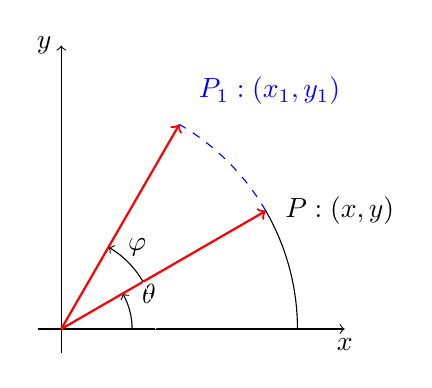
\begin{tikzpicture}[scale=3]
    % \draw[step=.5cm,gray,very thin] (-0.1,-0.1) grid (1.4,1.4);
    \draw[->] (-.1,0) -- (1.2,0)  node[below] {$x$};
    \draw[->] (0,-0.1) -- (0,1.2) node[left] {$y$};
    \draw[]   (1,0) arc (0:30:1) node(P)[label=right:$P:{(x,y)}$]{};
    \draw[->] (3mm,0mm) -- (3mm,0mm) arc (0:30:3mm) node(A)[label=right:$\theta$]{};
    \draw[red, thick, ->] (0,0) --  (P.center);
    
    \draw[white] (4mm,0mm) -- (4mm,0mm) arc (0:30:4mm) node(A){};
    \draw[->] (A.center) arc (30:60:4mm) node[label=right:$\varphi$]{};
    
    \draw[blue, dashed]  (P) arc (30:60:1) node(P1)[label=above right:$P_1:{(x_1,y_1)}$]{};
    
    \draw[red, thick, ->] (0,0) -- (P1.center);    
  \end{tikzpicture}
\end{figure}
这表明经过上述变换,将向量$OP$逆时针旋转$\varphi$角得到向量$OP_1$.


\begin{li}
  求解线性方程组
  $$
  \left\{
  \begin{array}{rcrcrcrcrr}
    2x_1 & - & 2x_2 &   &      & + &  6x_4 & = &-2 \\[0.1cm]
    2x_1 & - &  x_2 & + & 2x_3 & + &  4x_4 & = &-2 \\[0.1cm]
    3x_1 & - &  x_2 & + & 4x_3 & + &  4x_4 & = &-3 \\[0.1cm]
    5x_1 & - & 3x_2 & + &  x_3 & + & 20x_4 & = &-2 
  \end{array}
  \right.
  $$
\end{li}
\begin{jie}
  $$
  \left\{
  \begin{array}{rcrcrcrcrr}
    x_1 & - &  x_2 &   &      & + &  3x_4 & = &-1 \\[0.1cm]
    &  &  x_2 & + & 2x_3 & - &  2x_4 & = &0 \\[0.1cm]
    &  & 2x_2 & + & 4x_3 & - &  5x_4 & = &0 \\[0.1cm]
    &  & 2x_2 & + &  x_3 & + &  5x_4 & = &3 
  \end{array}
  \right.
  $$    
  $$
  \left\{
  \begin{array}{rcrcrcrcrr}
    x_1 & - &  x_2 &   &      & + &  3x_4 & = &-1 \\[0.1cm]
    &  &  x_2 & + & 2x_3 & - &  2x_4 & = &0 \\[0.1cm]
    &  &  &  &  & - &  x_4 & = &0 \\[0.1cm]
    &  &  & - &  3x_3 & + &  9x_4 & = &3 
  \end{array}
  \right.
  $$    
  $$
  \left\{
  \begin{array}{rcrcrcrcrr}
    x_1 & - &  x_2 &   &      & + &  3x_4 & = &-1 \\[0.1cm]
    &  &  x_2 & + & 2x_3 & - &  2x_4 & = &0 \\[0.1cm]
    &  &  & - &  3x_3 & + &  9x_4 & = &3 \\[0.1cm]
    &  &  &  &  & - &  x_4 & = &0 
  \end{array}
  \right.
  $$    
  $$
  \left\{
  \begin{array}{rcrcrcrcrr}
    x_1 & - &  x_2 &   &      & + &  3x_4 & = &-1 \\[0.1cm]
    &  &  x_2 & + & 2x_3 & - &  2x_4 & = &0 \\[0.1cm]
    &  &  &  &  x_3 & - &  3x_4 & = &-1 \\[0.1cm]
    &  &  &  &  &  &  x_4 & = &0 
  \end{array}
  \right.
  $$    
  如此形状的方程组称为\red{阶梯形线性方程组}.
  该方程组可写成矩阵形式
  \begin{figure}[htbp]
    \centering
    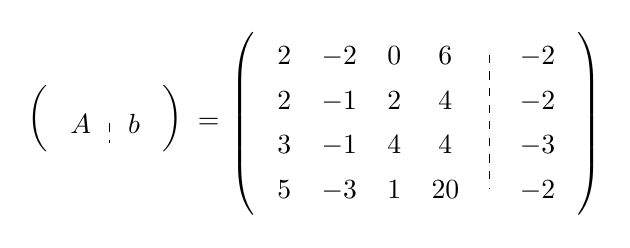
\begin{tikzpicture}
      \matrix(M) [matrix of math nodes,nodes in empty cells,,ampersand replacement=\&,left delimiter=(,right delimiter=)]{
        A \& \& b \\
      };
      \draw[dashed] (M-1-2.north) -- (M-1-2.south);
      \matrix(M1) [right=.1in of M,matrix of math nodes]{
        = \\
      };
      \matrix(MM) [right=.1in of M1,matrix of math nodes,nodes in empty cells,
        column sep=1ex,row sep=.5ex,ampersand replacement=\&,left delimiter=(,right delimiter=)] {
        2 \& -2 \& 0 \&  6 \& \& -2\\
        2 \& -1 \& 2 \&  4 \& \& -2\\
        3 \& -1 \& 4 \&  4 \& \& -3\\
        5 \& -3 \& 1 \& 20 \& \& -2\\
      };
      \draw[dashed] (MM-1-5.north) -- (MM-4-5);
    \end{tikzpicture}
    \caption{增广矩阵}
  \end{figure}
  求解过程可表示为
  \begin{figure}[htbp]
    \centering
    \begin{tikzpicture}          
      \matrix(A) [matrix of math nodes,nodes in empty cells,
        column sep=1ex,row sep=.1ex,ampersand replacement=\&,left delimiter=(,right delimiter=)] {
        A \& \& b \\
      };
      \draw[dashed] (A-1-2.north) -- (A-1-2.south);
      % \end{tikzpicture}
      
      % \begin{tikzpicture}
      \matrix (EQ1) [right=.1in of A,matrix of math nodes]  { 
        \xlongequal[]{\ds r_1 \div 2} \\
      };
      
      \matrix(A1) [right=.1in of EQ1,matrix of math nodes,nodes in empty cells, column sep=1ex,row sep=.1ex,ampersand replacement=\&,left delimiter=(,right delimiter=)] {
        1 \& -1 \& 0 \&  3 \& \& -1\\
        2 \& -1 \& 2 \&  4 \& \& -2\\
        3 \& -1 \& 4 \&  4 \& \& -3\\
        5 \& -3 \& 1 \& 20 \& \& -2\\
      };
      \draw[dashed] (A1-1-5.north) -- (A1-4-5);
      % \end{tikzpicture}

      
      % \begin{tikzpicture}
      
      \matrix(A2) [below=.1in of A1,matrix of math nodes,nodes in empty cells,
        column sep=1ex,row sep=.1ex,ampersand replacement=\&,left delimiter=(,right delimiter=)] {
        1 \& -1 \& 0 \&  3 \& \& -1\\
        0 \&  1 \& 2 \& -2 \& \&  0\\
        0 \&  0 \& 0 \& -1 \& \&  0\\
        0 \&  0 \&-3 \&  9 \& \&  3\\
      };
      \draw[dashed] (A2-1-5.north) -- (A2-4-5);
      \matrix (EQ2) [left=.1in of A2,matrix of math nodes]  { 
        \xlongequal[
          \ds r_3+(-3)\times r_1 \atop 
          \ds r_4+(-5)\times r_1]{\ds r_2+(-2)\times r_1} \\
      };

      % \end{tikzpicture}

      
      % \begin{tikzpicture}
      \matrix(A3) [below=.1in of A2,matrix of math nodes,nodes in empty cells,
        column sep=1ex,row sep=.1ex,ampersand replacement=\&,left delimiter=(,right delimiter=)] {
        1 \& -1 \& 0 \&  3 \& \& -1\\
        0 \&  1 \& 2 \& -2 \& \&  0\\
        0 \&  0 \&-3 \&  9 \& \&  3\\
        0 \&  0 \& 0 \& -1 \& \&  0\\
      };
      \draw[dashed] (A3-1-5.north) -- (A3-4-5);

      \matrix (EQ3) [left=.1in of A3,matrix of math nodes]  { 
        \xlongequal[]{\ds r_3 \leftrightarrow r_4} \\
      };

      
      \matrix(A4) [below=.1in of A3,matrix of math nodes,nodes in empty cells,
        column sep=1ex,row sep=.1ex,ampersand replacement=\&,left delimiter=(,right delimiter=)] {
        1 \& -1 \& 0 \&  3 \& \& -1\\
        0 \&  1 \& 2 \& -2 \& \&  0\\
        0 \&  0 \& 1 \& -3 \& \& -1\\
        0 \&  0 \& 0 \&  1 \& \&  0\\
      };
      \draw[dashed] (A4-1-5.north) -- (A4-4-5);

      \matrix (EQ4) [left=.1in of A4,matrix of math nodes]  { 
        \xlongequal[]{\ds r_3 \div (-3)} \\
      };
    \end{tikzpicture}
  \end{figure}
\end{jie}

\begin{li}
  求解线性方程组
  $$
  \left\{
  \begin{array}{rcrcrcrcrcrr}
    x_1 & - &  x_2 & - &  x_3 &   &       & + & 3x_5 & = &-1 \\[0.1cm]
    2x_1 & - & 2x_2 & - &  x_3 & + &  2x_4 & + & 4x_5 & = &-2 \\[0.1cm]
    3x_1 & - & 3x_2 & - &  x_3 & + &  4x_4 & + & 5x_5 & = &-3 \\[0.1cm]
    x_1 & - &  x_2 & + &  x_3 & + &   x_4 & + & 8x_5 & = & 2 
  \end{array}
  \right.
  $$
\end{li}
\newpage
\begin{jie}
  
  其增广矩阵为
  \begin{figure}[htbp]
    \centering
    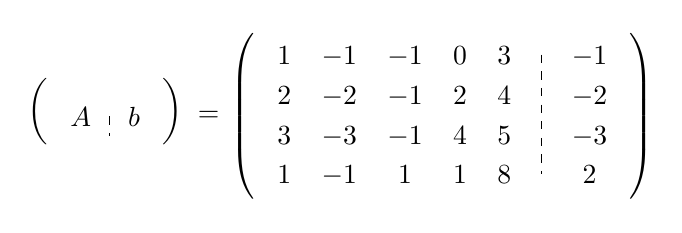
\begin{tikzpicture}
      \matrix(Ab) [matrix of math nodes,nodes in empty cells,,ampersand replacement=\&,left delimiter=(,right delimiter=)]{
        A \& \& b \\
      };
      \draw[dashed] (Ab-1-2.north) -- (Ab-1-2.south);
      \matrix (EQ) [right=.1in of Ab,matrix of math nodes]  { 
        =\\
      };
      \matrix(A) [right=.1in of EQ,matrix of math nodes,nodes in empty cells,   column sep=1ex,row sep=.1ex,ampersand replacement=\&,left delimiter=(,right delimiter=)] {
        1 \& -1 \& -1 \&  0 \& 3 \& \& -1\\
        2 \& -2 \& -1 \&  2 \& 4 \& \& -2\\
        3 \& -3 \& -1 \&  4 \& 5 \& \& -3\\
        1 \& -1 \&  1 \&  1 \& 8 \& \&  2\\
      };
      \draw[dashed] (A-1-6.north) -- (A-4-6);
    \end{tikzpicture}      
  \end{figure}
  
  求解过程可表示为:
  \begin{figure}[htbp]
    \centering
    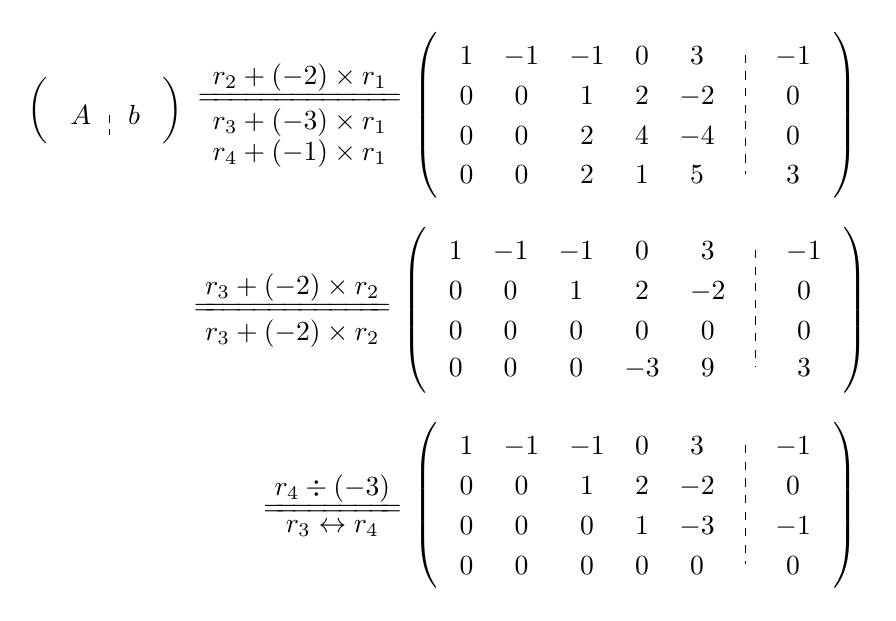
\begin{tikzpicture}
      \matrix(A) [matrix of math nodes,nodes in empty cells,,ampersand replacement=\&,left delimiter=(,right delimiter=)]{
        A \& \& b \\
      };
      \draw[densely dashed] (A-1-2.north) -- (A-1-2.south);
      \matrix (EQ1) [right=.1in of A,matrix of math nodes]  { 
        \xlongequal[\ds r_3+(-3)\times \ds r_1 \atop \ds r_4+(-1)\times r_1]{\ds r_2+(-2)\times r_1}\\
      };        
      \matrix(A1) [right=.1in of EQ1,matrix of math nodes,nodes in empty cells,
        column sep=1ex,row sep=.1ex,ampersand replacement=\&,left delimiter=(,right delimiter=)] {
        1 \& -1 \& -1 \&  0 \& 3 \& \& -1\\
        0 \&  0 \&  1 \&  2 \&-2 \& \&  0\\
        0 \&  0 \&  2 \&  4 \&-4 \& \&  0\\
        0 \&  0 \&  2 \&  1 \& 5 \& \&  3\\
      };
      \draw[dashed] (A1-1-6.north) -- (A1-4-6);

      \matrix(A2) [below=.1in of A1,matrix of math nodes,nodes in empty cells,
        column sep=1ex,row sep=.1ex,ampersand replacement=\&,left delimiter=(,right delimiter=)] {
        1 \& -1 \& -1 \&  0 \& 3 \& \& -1\\
        0 \&  0 \&  1 \&  2 \&-2 \& \&  0\\
        0 \&  0 \&  0 \&  0 \& 0 \& \&  0\\
        0 \&  0 \&  0 \& -3 \& 9 \& \&  3\\
      };
      \draw[dashed] (A2-1-6.north) -- (A2-4-6);
      \matrix (EQ2) [left=.1in of A2,matrix of math nodes]  { 
        \xlongequal[\ds r_3+(-2)\times r_2]{\ds r_3+(-2)\times r_2}\\
      };

      \matrix(A3) [below=.1in of A2,matrix of math nodes,nodes in empty cells,
        column sep=1ex,row sep=.1ex,ampersand replacement=\&,left delimiter=(,right delimiter=)] {
        1 \& -1 \& -1 \&  0 \& 3 \& \& -1\\
        0 \&  0 \&  1 \&  2 \&-2 \& \&  0\\
        0 \&  0 \&  0 \&  1 \& -3 \& \& -1\\
        0 \&  0 \&  0 \&  0 \& 0 \& \&  0\\
      };
      \draw[dashed] (A3-1-6.north) -- (A3-4-6);
      \matrix (EQ3) [left=.1in of A3,matrix of math nodes]  { 
        \xlongequal[\ds r_3 \leftrightarrow r_4]{\ds r_4\div(-3)}\\
      };
    \end{tikzpicture}           
  \end{figure}
  
  该矩阵称为\red{行简化阶梯矩阵},对应的线性方程组为
  $$
  \left\{
  \begin{array}{rcrcrcrcrcrr}
    x_1 & - &  x_2 &   &      &   &       & + & 7x_5 & = & 1 \\[0.1cm]
    &   &     &   &  x_3 &   &     & + & 4x_5 & = & 2 \\[0.1cm]
    &   &   &   &    &   &   x_4 & - & 3x_5 & = &-1
  \end{array}
  \right.
  $$
  \begin{zhu*}
    该方程组有$5$个未知量,其中$x_1,x_3,x_4$为\red{基本未知量},$x_2,x_5$为\red{自由未知量}。
  \end{zhu*}

  任取$x_2=k_1, x_5=k_2$,可得线性方程组的全部解
  $$
  \left\{
  \begin{array}{ccl}
    x_1 &=& 1+k_1-7k_2, \\[0.1cm]      
    x_2 &=& k_1, \\[0.1cm]
    x_3 &=& 2-4k_2, \\[0.1cm]
    x_4 &=& -1+3k_2,\\[0.1cm]
    x_5 &=& k_2.
  \end{array}
  \right.
  $$

\end{jie}

\begin{li}
  解线性方程组
  $$
  \left\{
  \begin{array}{rcrcrcr}
    x_1 & + & x_2 & + &  x_3 & = & 1, \\[0.1cm]
    x_1 & + &2x_2 & - & 5x_3 & = & 2, \\[0.1cm]
    2x_1 & + &3x_2 & - & 4x_3 & = & 5.
  \end{array}
  \right.
  $$
\end{li}
\newpage
\begin{jie}
  
  \begin{figure}[htbp]
    \centering
    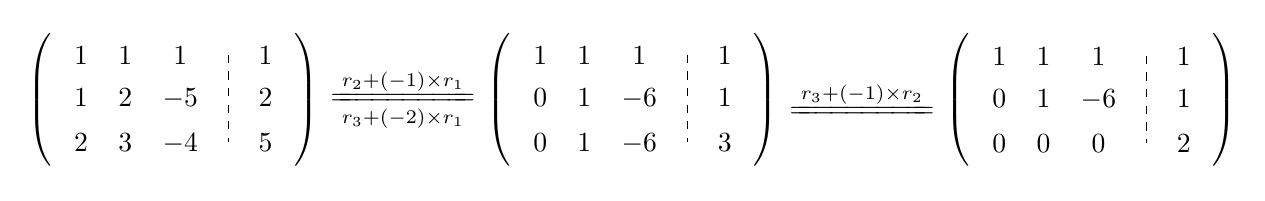
\begin{tikzpicture}        
      \matrix(Ab) [matrix of math nodes,nodes in empty cells,
        column sep=1ex,row sep=.5ex,ampersand replacement=\&,left delimiter=(,right delimiter=)] {
        1 \&  1 \&  1 \& \&  1\\
        1 \&  2 \& -5 \& \&  2\\
        2 \&  3 \& -4 \& \&  5\\
      };
      \draw[dashed] (Ab-1-4.north) -- (Ab-3-4);
      
      \matrix (EQ1) [right=.1in of Ab,matrix of math nodes]  { 
        \xlongequal[r_3+ (-2)\times r_1]{r_2+ (-1)\times r_1}\\
      };

      \matrix(Ab1) [right=.1in of EQ1,matrix of math nodes,nodes in empty cells, column sep=1ex,row sep=.5ex,ampersand replacement=\&,left delimiter=(,right delimiter=)] {
        1 \&  1 \&  1 \& \&  1\\
        0 \&  1 \& -6 \& \&  1\\
        0 \&  1 \& -6 \& \&  3\\
      };
      \draw[dashed] (Ab1-1-4.north) -- (Ab1-3-4);

      \matrix (EQ2) [right=.1in of Ab1,matrix of math nodes]  { 
        \xlongequal[]{r_3+ (-1)\times r_2}\\
      };
      \matrix(Ab2) [right=.1in of EQ2,matrix of math nodes,nodes in empty cells,column sep=1ex,row sep=.5ex,ampersand replacement=\&,left delimiter=(,right delimiter=)] {
        1 \&  1 \&  1 \& \&  1\\
        0 \&  1 \& -6 \& \&  1\\
        0 \&  0 \&  0 \& \&  2\\
      };
      \draw[dashed] (Ab2-1-4.north) -- (Ab2-3-4);        
    \end{tikzpicture}
  \end{figure}
  
  由第三行可以看出,该线性方程组无解。
\end{jie}

\begin{itemize}
\item 含有矛盾方程而无解的方程组称为\red{不相容方程组};
\item 有解的方程组称为\red{相容方程组};
\item \red{多余方程}。
\end{itemize}

对于一般的线性方程组
$$
\left\{
\begin{array}{c}
  a_{11}x_1 + a_{12}x_2 + \cd + a_{1n}x_n = b_1\\[0.2cm]
  a_{21}x_1 + a_{22}x_2 + \cd + a_{2n}x_n = b_2\\[0.2cm]
  \vd\\[0.2cm]
  a_{m1}x_1 + a_{m2}x_2 + \cd + a_{mn}x_n = b_m
\end{array}
\right.
$$

其增广矩阵为
\begin{figure}[htbp]
  \centering
  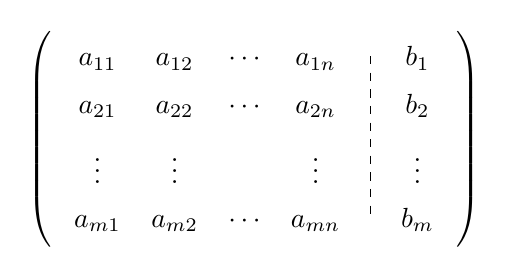
\begin{tikzpicture}
    \matrix(MM) [matrix of math nodes,nodes in empty cells,
      column sep=1ex,row sep=.5ex,ampersand replacement=\&,left delimiter=(,right delimiter=)] {
      a_{11} \&  a_{12} \&  \cd \& a_{1n} \& \&  b_1\\
      a_{21} \&  a_{22} \&  \cd \& a_{2n} \& \&  b_2\\
      \vd   \&  \vd   \&      \&  \vd  \& \& \vd \\
      a_{m1} \&  a_{m2} \&  \cd \& a_{mn} \& \&  b_m\\
    };
    \draw[dashed] (MM-1-5.north) -- (MM-4-5);        
  \end{tikzpicture}      
\end{figure}
对于以上增广矩阵,总是可以经过一系列的变换将其化成
\begin{figure}[htbp]
  \centering
  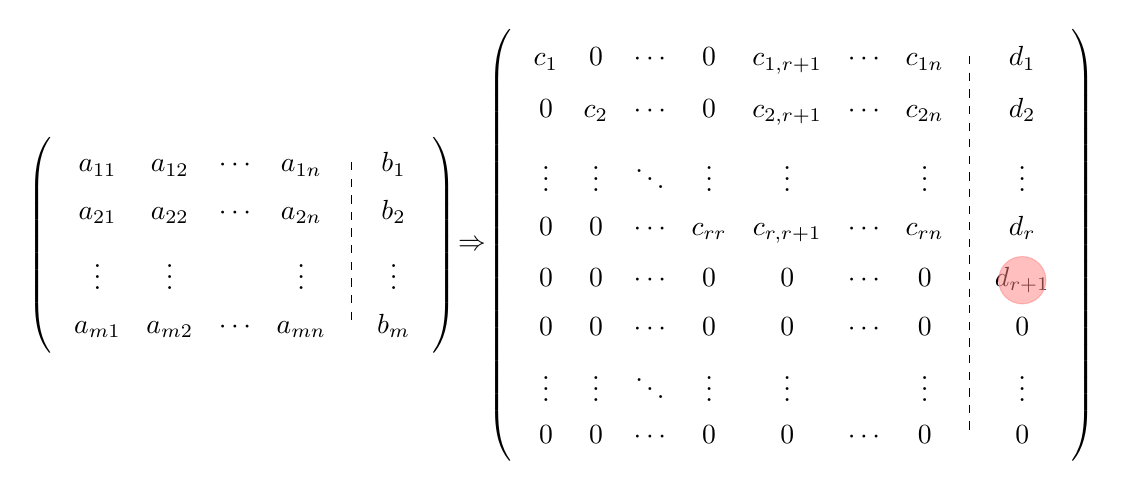
\begin{tikzpicture}
    \matrix(MM) [matrix of math nodes,nodes in empty cells,
      column sep=0.6ex,row sep=.5ex,ampersand replacement=\&,left delimiter=(,right delimiter=)] {
      a_{11} \&  a_{12} \&  \cd \& a_{1n} \& \&  b_1\\
      a_{21} \&  a_{22} \&  \cd \& a_{2n} \& \&  b_2\\
      \vd   \&  \vd   \&      \&  \vd  \& \& \vd \\
      a_{m1} \&  a_{m2} \&  \cd \& a_{mn} \& \&  b_m\\
    };
    \draw[dashed] (MM-1-5.north) -- (MM-4-5);
    
    \matrix (M2) [right=.05in of MM,matrix of math nodes]  { 
      \Rightarrow\\
    };
    
    \matrix(MM) [right=.05in of M2,matrix of math nodes,nodes in empty cells,
      column sep=0.6ex,row sep=.5ex,ampersand replacement=\&,left delimiter=(,right delimiter=)] {
      c_1 \&   0 \& \cd \&  0 \& c_{1,r+1} \& \cd \& c_{1n} \& \& d_1\\
      0   \& c_2 \& \cd \&  0 \& c_{2,r+1} \& \cd \& c_{2n} \& \& d_2\\
      \vd \& \vd \& \dd \&\vd \& \vd     \&     \& \vd   \& \& \vd\\
      0   \&  0  \& \cd \& c_{rr} \& c_{r,r+1} \& \cd \& c_{rn} \& \& d_r\\
      0   \&  0  \& \cd \& 0 \& 0 \& \cd \& 0 \&  \& d_{r+1}\\
      0   \&  0  \& \cd \& 0 \& 0 \& \cd \& 0 \&  \& 0\\          
      \vd \& \vd \& \dd \&\vd \& \vd     \&     \& \vd   \& \& \vd\\
      0   \&  0  \& \cd \& 0 \& 0 \& \cd \& 0 \&  \& 0\\
    };
    \draw[dashed] (MM-1-8.north) -- (MM-8-8);
    \filldraw[opacity=0.5,red!50] (MM-5-9) circle (0.3cm);
  \end{tikzpicture}      
\end{figure}
其中$c_{ii}=1~(i=1,2,\cd,r)$。对应线性方程组解的情况如下:   
\begin{itemize}
\item[1] 线性方程组有解$ \Leftrightarrow \red{d_{r+1}=0}$;\\[0.3cm]
\item[2] 在有解的情况下:
  \begin{itemize}
  \item 当$r=n$时,有唯一解$x_1=d_1,~x_2=d_2,~\cd,~x_n=d_n$;
  \item 当$r<n$时,有无穷多解
    $$
    \left\{
    \begin{array}{ccl}
      x_1 &=& d_1 - c_{1,r+1}k_1 - \cd - c_{1n}k_{n-r}, \\[0.1cm]
      x_2 &=& d_2 - c_{2,r+1}k_1 - \cd - c_{2n}k_{n-r}, \\[0.1cm]
      \vd & & \vd \\[0.1cm]
      x_r &=& d_r - c_{r,r+1}k_1 - \cd - c_{rn}k_{n-r}, \\[0.1cm]
      x_{r+1} &=& k_1, \\[0.1cm]
      \vd && \vd \\[0.1cm]
      x_{n} &=& k_{n-r}.
    \end{array}
    \right.
    $$
  \end{itemize}
\end{itemize}

  %%%% 
\section{矩阵的计算}
\subsection{矩阵的加法}
\begin{frame}
  \begin{footnotesize}
    
    \begin{block}{矩阵的加法}
      设有两个$m\times n$矩阵$\A=(a_{ij})$和$\B=(b_{ij})$,则矩阵$\A$与$\B$之和记为$\A+\B$,规定为
      $$
      \A + \B = 
      \left(
        \begin{array}{cccc}
          a_{11} + b_{11}  & a_{12} + b_{12}  & \cd & a_{1n} + b_{1n}  \\[0.2cm]
          a_{21} + b_{21}  & a_{22} + b_{22}  & \cd & a_{2n} + b_{2n}  \\[0.2cm]
          \cd            & \cd            &     & \cd            \\[0.2cm]
          a_{n1} + b_{n1}  & a_{n2} + b_{n2}  & \cd & a_{nn} + b_{nn}  
        \end{array}
      \right)
      $$
    \end{block}
    \pause
    \begin{block}{注}
      \red{只有当两个矩阵同型时才能进行加法运算。}
    \end{block}

    


  \end{footnotesize}
\end{frame}


\begin{frame}
  \begin{footnotesize}
    \begin{block}{矩阵加法运算律}
      \begin{itemize}
      \item[(i)] $\A + \B = \B + \A$\\[0.2cm]
      \item[(ii)] $(\A + \B) + \C = \A + (\B + \C)$ 
      \end{itemize}
    \end{block}

    \vspace{0.1in}
    \pause 
    设$\A = (a_{ij})$,称
    $$
    -\A = (-a_{ij}),
    $$
    为$\A$的负矩阵,显然有
    $$
    \A + (-\A) = \mathbf{0}.
    $$
    由此规定矩阵的减法为
    $$
    \A - \B = \A + (-\B).
    $$
  \end{footnotesize}
\end{frame}

\subsection{矩阵的数乘}
\begin{frame}
  \begin{footnotesize}
    \begin{block}{矩阵的数乘}
      数$k$与矩阵$\A$的乘积记作$k \A$或$\A k$,规定为
      $$
      k \A = 
      \left(
        \begin{array}{cccc}
          k a_{11}   & k a_{12}   & \cd & k a_{1n}  \\[0.2cm]
          k a_{21}   & k a_{22}   & \cd & k a_{2n}  \\[0.2cm]
          \cd     & \cd     &     & \cd    \\[0.2cm]
          k a_{m1}   & k a_{m2}   & \cd & k a_{mn}  
        \end{array}
      \right)
      $$
    \end{block}
    \pause 
    \begin{block}{注}
      \red{用数$k$乘一个矩阵,需要把数$k$乘矩阵的每一个元素,这与行列式的数乘性质不同。}
    \end{block}
  \end{footnotesize}
\end{frame}


\begin{frame}
  \begin{footnotesize}
    \begin{block}{矩阵数乘运算律}
      \begin{itemize}
      \item[(i)] $(k l)\A =  k(l \A)$\\[0.2cm]
      \item[(ii)] $(k + l) \A  = k \A + l \A$\\[0.2cm]
      \item[(iii)] $k (\A + \B)  = k \A + k \B$
      \end{itemize}
    \end{block}
    \pause 
    \purple{矩阵加法与矩阵数乘统称为矩阵的线性运算}
  \end{footnotesize}
\end{frame}


\subsection{矩阵的乘法}
\begin{frame}
  \begin{footnotesize}
    设有两个线性变换
    \begin{equation}\label{lt1}
      \left\{
        \begin{array}{l}
          y_1 = a_{11} x_1 + a_{12} x_2 + a_{13} x_3, \\[0.2cm]
          y_2 = a_{21} x_1 + a_{22} x_2 + a_{23} x_3,
        \end{array}
      \right.
    \end{equation}
    \pause
    \begin{equation}\label{lt2}
      \left\{
        \begin{array}{l}
          x_1 = b_{11} t_1 + b_{12} t_2 , \\[0.2cm]
          x_2 = b_{21} t_1 + b_{22} t_2 , \\[0.2cm]
          x_3 = b_{31} t_1 + b_{32} t_2 , 
        \end{array}
      \right.
    \end{equation}
    \pause
    若想求从$t_1, t_2$到$y_1, y_2$的线性变换,可将(\ref{lt2})代入(\ref{lt1}),便得
    \begin{equation}\label{lt3}
      \left\{
        \begin{array}{l}
          y_1 = (a_{11}b_{11} + a_{12}b_{21} + a_{13}b_{31}) t_1 + (a_{11}b_{12} + a_{12}b_{22} + a_{13}b_{32})t_2, \\[0.2cm]
          y_2 = (a_{21}b_{11} + a_{22}b_{21} + a_{23}b_{31}) t_1 + (a_{21}b_{12} + a_{22}b_{22} + a_{23}b_{32})t_2.
        \end{array}
      \right.
    \end{equation}
    \pause
    \red{线性变换(\ref{lt3})可看成是先作线性变换(\ref{lt2})再作线性变换(\ref{lt1})的结果}。
  \end{footnotesize}
\end{frame}

\begin{frame}
  \begin{footnotesize}
    把线性变换(\ref{lt3})叫做线性变换(\ref{lt1})和(\ref{lt2})的乘积,
    相应地把线性变换(\ref{lt3})对应的矩阵定义为线性变换(\ref{lt1})与(\ref{lt2})所对应矩阵的乘积,即
    $$
    \begin{array}{ll}
      & \left(
        \begin{array}{lll}
          a_{11} & a_{12} & a_{13}\\[0.1cm]
          a_{21} & a_{22} & a_{23}
        \end{array}
                            \right)
                            \left(
                            \begin{array}{ll}
                              b_{11} & b_{12} \\[0.1cm]
                              b_{21} & b_{22} \\[0.1cm]
                              b_{31} & b_{32} 
                            \end{array}
                                       \right) \\[0.8cm]
      = & \left(
          \begin{array}{cc}
            a_{11}b_{11} + a_{12}b_{21} + a_{13}b_{31}  &  a_{11}b_{12} + a_{12}b_{22} + a_{13}b_{32} \\[0.1cm]
            a_{21}b_{11} + a_{22}b_{21} + a_{23}b_{31}  &  a_{21}b_{12} + a_{22}b_{22} + a_{23}b_{32}
          \end{array}
                                                          \right)
    \end{array}
    $$
  \end{footnotesize}
\end{frame}

\begin{frame}
  \begin{footnotesize}
    \begin{block}{矩阵乘法}
      设$A$为$m\times n$矩阵,$B$为$n\times s$矩阵,即
      $$
      A = \left(
        \begin{array}{cccc}
          a_{11} & a_{12} & \cd & a_{1n}\\
          a_{21} & a_{22} & \cd & a_{2n}\\
          \vd   & \vd   &     & \vd \\
          a_{m1} & a_{m2} & \cd & a_{mn}
        \end{array}
      \right), ~~
      B = \left(
        \begin{array}{cccc}
          b_{11} & b_{12} & \cd & b_{1s}\\
          b_{21} & b_{22} & \cd & b_{2s}\\
          \vd   & \vd   &     & \vd \\
          b_{n1} & b_{n2} & \cd & b_{ns}
        \end{array}
      \right)
      $$
      则$A$与$B$之乘积$AB$(记为$C=(c_{ij})$)为$m\times s$矩阵,且
      $$
      c_{ij} = c_{i1}b_{1j} + c_{i2}b_{2j} + \cd + c_{in}b_{nj} = \sum_{k=1}^na_{ik}b_{kj}.
      $$
    \end{block}
    \pause 
    \begin{block}{注}
      两个矩阵$A$与$B$相乘有意义的前提是\red{$A$的列数等于$B$的行数}。
    \end{block}
  \end{footnotesize}
\end{frame}


\begin{frame}
  % l' unite
  \newcommand{\myunit}{0.5 cm}
  \tikzset{
    node style sp/.style={draw,circle,minimum size=\myunit},
    node style ge/.style={circle,minimum size=\myunit},
    arrow style mul/.style={draw,sloped,midway,fill=white},
    arrow style plus/.style={midway,sloped,fill=white},
  }
  
  \begin{tikzpicture}[scale=0.5,>=latex]
    % les matrices
    \matrix (A) [matrix of math nodes,%
    nodes = {node style ge},%
    ampersand replacement=\&,
    left delimiter  = (,%
    right delimiter = )] at (0,0)   {%
      a_{11} \& a_{12} \& \ldots \& a_{1n}  \\
      \blue{a_{21}}  \& \blue{a_{22}}; \& \ldots%
      \& \blue{a_{2n}} \\
      \vdots \& \vdots \& \ddots \& \vdots  \\
      a_{m1} \& a_{m2} \& \ldots \& a_{mn}  \\
    };
    \pause 
    % \node [draw,below=1pt] at (A.south) { 
    % $A$ : \textcolor{red}{$n$ rows} $p$ columns};

    \matrix (B) [matrix of math nodes,%
    % nodes = {node style ge},%
    ampersand replacement=\&,
    left delimiter  = (,%
    right delimiter =)] at (20*\myunit,18*\myunit){%
      b_{11} \& \blue{b_{12}}%
      \& \ldots \& b_{1s}  \\
      b_{21} \& \blue{b_{22}}%
      \& \ldots \& b_{2s}  \\
      \vdots \& \vdots \& \ddots \& \vdots  \\
      b_{n1} \& \blue{b_{n2}}%
      \& \ldots \& b_{ns}  \\
    };
    \pause
    %% \node [draw,above=10pt] at (B.north) { 
    %% $B$ : $p$ rows \textcolor{red}{$q$ columns}
    %% };
    %   matrice 
    \matrix (C) [matrix of math nodes,%
    nodes = {node style ge},%
    ampersand replacement=\&,
    left delimiter  = (,%
    right delimiter = )] at (20*\myunit,0) {%
      c_{11} \& c_{12} \& \ldots \& c_{1s} \\
      c_{21} \& \red{c_{22}}%
      \& \ldots \& c_{2s} \\
      \vdots \& \vdots \& \ddots \& \vdots \\
      c_{m1} \& c_{m2} \& \ldots \& c_{ms} \\
    };
    \pause 
    % les fleches
    \draw[<->,red](A-2-1) to[in=180,out=90]
    node[arrow style mul] (x) {$a_{21}\times b_{12}$} (B-1-2);
    \pause 
    \draw[<->,red](A-2-2) to[in=180,out=90]
    node[arrow style mul] (y) {$a_{22}\times b_{22}$} (B-2-2);
    \pause 
    \draw[<->,red](A-2-4) to[in=180,out=90]
    node[arrow style mul] (z) {$a_{2n}\times b_{n2}$} (B-4-2);
    \pause 
    \draw[red,->] (x) to node[arrow style plus] {$+$} (y)%
    to node[arrow style plus] {$+\raisebox{.5ex}{\ldots}+$} (z)%
    to (C-2-2.north west);
    \pause 
    \draw[blue] (A-2-1.north) -- (C-2-2.north);
    \draw[blue] (A-2-1.south) -- (C-2-2.south);

    \draw[blue] (B-1-2.west)  -- (C-2-2.west);
    \draw[blue] (B-1-2.east)  -- (C-2-2.east);

    %% \node [draw,below=10pt] at (C.south) 
    %% {$ C=A\times B$ : \textcolor{red}{$n$ rows}  \textcolor{red}{$q$ columns}};

  \end{tikzpicture}

\end{frame}

\begin{frame}
  \begin{footnotesize}
    \begin{exampleblock}{例1}
      求矩阵
      $
      \A = \left(
        \begin{array}{rrrr}
          1&2&-1\\
          -1&3&4\\
          1&1&1
        \end{array}
      \right)
      $
      与
      $
      \B = \left(
        \begin{array}{rrrr}
          5&6\\
          -5&-6\\
          6&0
        \end{array}
      \right)
      $
      的乘积$\A\B$
    \end{exampleblock}
    \pause
    \textbf{解:}
    $$
    \begin{array}{cl}
      \A\B &\pause = \left(
             \begin{array}{ccc}
               1\times5 + 2\times(-5) + (-1)\times6 &
                                                      1\times6 + 2\times(-6) + (-1)\times0 \\[0.1cm]
               (-1)\times5 + 3\times(-5) +    4\times6 &
                                                         (-1)\times6 + 3\times(-6) +    4\times0 \\[0.1cm]
               1\times5 + 1\times(-5) +    1\times6 &
                                                      1\times6 + 1\times(-6) +    1\times0 
             \end{array}
                                                      \right) \\[0.3in]
           &\pause =\left(
             \begin{array}{rr}
               -11 & -6\\
               4 & -24\\
               6 & 0
             \end{array}
                   \right)   
    \end{array}
    $$
  \end{footnotesize}
\end{frame}

\begin{frame}
  \begin{footnotesize}
    \begin{exampleblock}{例2}
      设
      $$
      \A = \left(
        \begin{array}{c}
          a_1\\
          a_2\\
          \vd\\
          a_n
        \end{array}
      \right), ~~
      \B = \left(
        \begin{array}{cccc}
          b_1 & b_2 & \cd & b_n
        \end{array}
      \right)
      $$
      计算$\A\B$与$\B\A$.
    \end{exampleblock}
    \textbf{解:}
    $$
    \A\B = \left(
      \begin{array}{c}
        a_1\\
        a_2\\
        \vd\\
        a_n
      \end{array}
    \right)\left(
      \begin{array}{cccc}
        b_1 & b_2 & \cd & b_n
      \end{array}
    \right)\pause 
    = \left(
      \begin{array}{cccc}
        a_1b_1 & a_1b_2 & \cd & a_1b_n\\
        a_2b_1 & a_2b_2 & \cd & a_2b_n\\
        \vd & \vd & & \vd\\
        a_nb_1 & a_nb_2 & \cd & a_nb_n
      \end{array}
    \right)
    $$ \pause 
    $$
    \B\A = \left(
      \begin{array}{cccc}
        b_1 & b_2 & \cd & b_n
      \end{array}
    \right)\left(
      \begin{array}{c}
        a_1\\
        a_2\\
        \vd\\
        a_n
      \end{array}
    \right) \pause 
    = a_1b_1+a_2b_2+\cd+a_nb_n.
    $$
  \end{footnotesize}
\end{frame}

\begin{frame}
  \begin{footnotesize}
    \begin{exampleblock}{例3}
      设
      $$
      \A = \left(
        \begin{array}{cc}
          a & a\\
          -a & -a
        \end{array}
      \right), ~
      \B = \left(
        \begin{array}{cc}
          b & -b\\
          -b & b
        \end{array}
      \right),~
      \C = \left(
        \begin{array}{cc}
          -1 & 1\\
          1 & -1
        \end{array}
      \right)
      $$
      计算$\A\B, ~\A\C$和$\B\A$.
    \end{exampleblock}
    \pause
    \textbf{解:}
    $$
    \A\B = \A\C = \left(
      \begin{array}{cc}
        0 & 0\\
        0 & 0
      \end{array}
    \right)
    $$\pause
    $$
    \B\A = \left(
      \begin{array}{cc}
        2ab & 2ab\\
        -2ab & -2ab
      \end{array}
    \right)
    $$      
  \end{footnotesize}
\end{frame}


\begin{frame}
  \begin{footnotesize}
    由以上例题可以看出一些结论:\pause 
    \begin{itemize}
    \item[1] 矩阵乘法不满足交换律。\\[0.2cm] \pause 
    \item[] 若$\A\B\ne\B\A$,则称\red{$\A$与$\B$不可交换}。\\[0.2cm] \pause 
    \item[] 若$\A\B=\B\A$,则称\red{$\A$与$\B$可交换}。  \\[0.4cm] \pause 
    \item[2] $\A\B=\zero ~\nRightarrow~ \A = \zero \mbox{或} \B = \zero$\\[0.2cm] \pause 
    \item[]  $\A\ne\zero\mbox{且} \B\ne\zero ~\xLongrightarrow[]{\mbox{有可能}}~ \A \B= \zero$\\[0.4cm] \pause
    \item[3] 矩阵乘法不满足消去律,即当$\A\ne\zero$时,
      $$
      \A\B=\A\C ~\nRightarrow~ \B=\C
      $$\\[0.2cm] \pause 
    \item[]当$\A$为非奇异矩阵,即$|\A|\ne 0$时,
      $$
      \A\B=\zero ~\Rightarrow~ \B = \zero; ~~~
      \A\B=\A\C ~\Rightarrow~ \B = \C.
      $$
    \end{itemize}
  \end{footnotesize}
\end{frame}


\begin{frame}
  \begin{footnotesize}
    \begin{block}{矩阵乘法运算律}
      \begin{itemize}
      \item[(i)] 结合律
      \item[] $$ (\A\B)\C = \A(\B\C)$$
      \item[(ii)] 数乘结合律
      \item[] $$ k(\A\B) = (k\A)\B = \A(k\B)$$
      \item[(iii)] 左结合律
      \item[] $$ \A(\B+\C) = \A\B+\A\C$$
      \item[] 右结合律
      \item[] $$ (\B+\C)\A = \B\A+\C\A$$
        
      \end{itemize}
    \end{block}
  \end{footnotesize}
\end{frame}

\subsection{一些特殊矩阵及其运算}
\begin{frame}
  \begin{footnotesize}
    \begin{block}{单位矩阵与数量矩阵}
      \begin{itemize}
      \item[1] 主对角元全为1,其余元素全为零的$n$阶方阵,称为$n$阶\red{单位矩阵},记为$\II_n, \II, \E$
        $$
        \II_n = \left(
          \begin{array}{cccc}
            1 & & &\\
              & 1 & & \\
              & & \dd & \\
              & & & 1
          \end{array}
        \right)
        $$\pause 
      \item[2] 主对角元全为非零数$k$,其余元素全为零的$n$阶方阵,称为$n$阶\red{数量矩阵},记为$k\II_n, k\II, k\E$
        $$
        k\II_n = \left(
          \begin{array}{cccc}
            k & & &\\
              & k & & \\
              & & \dd & \\
              & & & k
          \end{array}
        \right)~(k\ne 0)
        $$
      \end{itemize}
    \end{block}
    \pause 
    \begin{block}{注}
      \begin{itemize}
      \item[1] \red{单位阵在矩阵乘法中的作用相当于数$1$在数的乘法中的作用。}\\ \pause 
      \item[2] 
        $$
        (k\II) \A = k(\II\A) = k\A, ~~
        \A(k\II) = k(\A\II) = k\A.
        $$
      \end{itemize}
    \end{block}
  \end{footnotesize}
\end{frame}


\begin{frame}
  \begin{footnotesize}
    \begin{block}{对角矩阵}
      非对角元皆为零的$n$阶方阵称为$n$阶\red{对角矩阵},记作$\LLambda$,即
      $$
      \LLambda = \left(
        \begin{array}{cccc}
          \lambda_1 & & &\\
                    & \lambda_2 & & \\
                    & & \dd & \\
                    & & & \lambda_n
        \end{array}
      \right)
      $$
      或记作$\mathrm{diag}(\lambda_1,\lambda_2,\cd,\lambda_n)$.
    \end{block}
  \end{footnotesize}
\end{frame}


\begin{frame}
  \begin{footnotesize}
    \begin{block}{注}
      \begin{itemize}
      \item[1] 用对角阵$\LLambda$左乘$\A$,就是用$\lambda_i(i=1,\cd,n)$乘$\A$中第$i$行的每个元素;
        \pause 
      \item[]
        \begin{scriptsize}
          $$
          \left(
            \begin{array}{cccc}
              \lambda_1 & & &\\
                        & \lambda_2 & & \\
                        & & \dd & \\
                        & & & \lambda_n
            \end{array}
          \right)
          \left(
            \begin{array}{cccc}
              a_{11} & a_{12} & \cd & a_{1n}\\
              a_{21} & a_{22} & \cd & a_{2n}\\
              \vd & \vd &  & \vd\\
              a_{n1} & a_{n2} & \cd & a_{nn}
            \end{array}
          \right) = 
          \left(
            \begin{array}{cccc}
              \lambda_1 a_{11} & \lambda_1a_{12} & \cd & \lambda_1a_{1n}\\
              \lambda_2a_{21} & \lambda_2a_{22} & \cd & \lambda_2a_{2n}\\
              \vd & \vd &  & \vd\\
              \lambda_na_{n1} & \lambda_na_{n2} & \cd & \lambda_na_{nn}
            \end{array}
          \right)
          $$

        \end{scriptsize}
        \pause 
      \item[2] 用对角阵$\LLambda$右乘$\A$,就是用$\lambda_i(i=1,\cd,n)$乘$\A$中第$i$列的每个元素;
        \pause 
      \item[]
        \begin{scriptsize}
          $$
          \left(
            \begin{array}{cccc}
              a_{11} & a_{12} & \cd & a_{1n}\\
              a_{21} & a_{22} & \cd & a_{2n}\\
              \vd & \vd &  & \vd\\
              a_{n1} & a_{n2} & \cd & a_{nn}
            \end{array}
          \right)  
          \left(
            \begin{array}{cccc}
              \lambda_1 & & &\\
                        & \lambda_2 & & \\
                        & & \dd & \\
                        & & & \lambda_n
            \end{array}
          \right)
          = 
          \left(
            \begin{array}{cccc}
              \lambda_1a_{11} & \lambda_2a_{12} & \cd & \lambda_na_{1n}\\
              \lambda_1a_{21} & \lambda_2a_{22} & \cd & \lambda_na_{2n}\\
              \vd & \vd &  & \vd\\
              \lambda_1a_{n1} & \lambda_2a_{n2} & \cd & \lambda_na_{nn}
            \end{array}
          \right)
          $$

        \end{scriptsize}
      \end{itemize}
    \end{block}
  \end{footnotesize}
\end{frame}


\begin{frame}
  \begin{footnotesize}
    \begin{block}{三角矩阵}
      \begin{itemize}
      \item[1] 主对角线以上的元素全为零的$n$阶方阵称为\red{上三角矩阵}($a_{ij}=0, ~i>j$)
        $$
        \left(
          \begin{array}{cccc}
            a_{11} & a_{12} & \cd & a_{1n} \\
                   & a_{22} & \cd & a_{2n} \\
                   &       & \dd & \vd   \\
                   &       &     & a_{nn}
          \end{array}
        \right)
        $$
      \item[2] 主对角线以下的元素全为零的$n$阶方阵称为\red{下三角矩阵}($a_{ij}=0, ~i<j$)
        $$
        \left(
          \begin{array}{cccc}
            a_{11} &       &     &       \\
            a_{21} & a_{22} &     &  \\
            \vd   & \vd   & \dd &    \\
            a_{n1} & a_{n2} & \cd & a_{nn}
          \end{array}
        \right)
        $$
      \end{itemize}
    \end{block}
  \end{footnotesize}
\end{frame}

\begin{frame}
  \begin{footnotesize}
    \begin{exampleblock}{例4}
      证明:两个上三角矩阵的乘积仍为上三角矩阵。
    \end{exampleblock}
    \proofname
    设
    $$
    \A = \left(
      \begin{array}{cccc}
        a_{11} & a_{12} & \cd & a_{1n} \\
               & a_{22} & \cd & a_{2n} \\
               &       & \dd & \vd   \\
               &       &     & a_{nn}
      \end{array}
    \right), ~     \B = \left(
      \begin{array}{cccc}
        b_{11} & b_{12} & \cd & b_{1n} \\
               & b_{22} & \cd & b_{2n} \\
               &       & \dd & \vd   \\
               &       &     & b_{nn}
      \end{array}
    \right)
    $$
    \pause 
    令$\C = \A\B = (c_{ij})$,
    则当$i>j$时,
    $$
    c_{ij} = \sum_{k=1}^n a_{ik}b_{kj}  \pause 
    = \sum_{k=1}^{i-1} a_{ik}b_{kj}  + \sum_{k=i}^n a_{ik}b_{kj} \pause 
    = \sum_{k=1}^{i-1} \red{\underbrace{a_{ik}}_{\Downarrow\atop0}}b_{kj}  
    + \sum_{k=i}^n a_{ik}\red{\underbrace{b_{kj}}_{\Downarrow\atop0}} \pause = 0.
    $$
    \pause 
    \begin{block}{注}
      两个下三角矩阵的乘积仍是下三角矩阵。
    \end{block}
  \end{footnotesize}
\end{frame}


\begin{frame}
  \begin{footnotesize}
    设线性方程组
    $$
    \left\{
      \begin{array}{c}
        a_{11}x_1 + a_{12}x_2 + a_{1n}x_n = b_1, \\[0.2cm]
        a_{21}x_1 + a_{22}x_2 + a_{2n}x_n = b_2, \\[0.2cm]
        \vd \\[0.2cm]
        a_{m1}x_1 + a_{m2}x_2 + a_{mn}x_n = b_m.
      \end{array}
    \right.
    $$
    \pause
    第$i$个方程可表示为
    $$
    \left(
      \begin{array}{cccc}
        a_{i1} & a_{i2} & \cd &  a_{in}
      \end{array}
    \right)
    \left(
      \begin{array}{c}
        x_{1} \\
        x_{2} \\
        \cd   \\
        x_{n}
      \end{array}
    \right) = b_i, \quad i=1,2,\cd,n.
    $$\pause 
    因此上述线性方程组可表示为
    $$
    \underbrace{
      \left(
        \begin{array}{cccc}
          a_{11} & a_{12} & \cd &  a_{1n} \\[0.1cm]
          a_{21} & a_{22} & \cd &  a_{2n} \\[0.1cm]
          \vd   & \vd   &     & \vd \\[0.1cm]
          a_{n1} & a_{n2} & \cd &  a_{nn} \\[0.1cm]
        \end{array}
      \right)
    }_{\red{\A}}
    \underbrace{
      \left(
        \begin{array}{c}
          x_{1} \\[0.1cm]
          x_{2} \\[0.1cm]
          \vd  \\[0.1cm]
          x_{n}
        \end{array}
      \right)
    }_{\red{\xx}}
    =     
    \underbrace{
      \left(
        \begin{array}{c}
          b_{1} \\[0.1cm]
          b_{2} \\[0.1cm]
          \vd  \\[0.1cm]
          b_{n}
        \end{array}
      \right)
    }_{\red{\bb}},  
    \pause \quad \red{\A\xx=\bb}.
    $$
  \end{footnotesize}
\end{frame}


\begin{frame}
  \begin{footnotesize}
    \begin{block}{定理}
      设$\A,\B$是两个$n$阶方阵,则
      $$
      |\A\B| = |\A||\B|.
      $$
    \end{block}
    \pause 
    \proofname
    设$\A=(a_{ij})_{n\times n}, ~\B=(b_{ij})_{n\times n}$,则
    $$
    |\A||\B| = \left|
      \begin{array}{cccccccc}
        a_{11} & a_{12} & \cd &  a_{1n} & 0 & 0 & \cd & 0\\
        a_{21} & a_{22} & \cd &  a_{2n} & 0 & 0 & \cd & 0\\
        \vd   & \vd   &     & \vd    & \vd & \vd & & \vd\\
        a_{n1} & a_{n2} & \cd &  a_{nn} & 0 & 0 & \cd & 0\\
        -1    & 0     & \cd &   0    & b_{11} & b_{12} & \cd & b_{1n} \\
        0 & -1 & \cd & 0& b_{21} & b_{22} & \cd & b_{2n} \\
        \vd&\vd & & \vd &  \vd  &\vd &  & \vd   \\
        0 & 0 & \cd & -1 & b_{n1} & b_{n2} &\cd     & b_{nn}
      \end{array}
    \right|
    $$
    
  \end{footnotesize}
\end{frame}

\begin{frame}
  \begin{footnotesize}
    $$
    \begin{array}{rl}
      & \left|
        \begin{array}{cccccccc}
          a_{11} & a_{12} & \cd &  a_{1n} & 0 & 0 & \cd & 0\\
          a_{21} & a_{22} & \cd &  a_{2n} & 0 & 0 & \cd & 0\\
          \vd   & \vd   &     & \vd    & \vd & \vd & & \vd\\
          a_{n1} & a_{n2} & \cd &  a_{nn} & 0 & 0 & \cd & 0\\
          -1    & 0     & \cd &   0    & b_{11} & b_{12} & \cd & b_{1n} \\
          0 & -1 & \cd & 0& b_{21} & b_{22} & \cd & b_{2n} \\
          \vd&\vd & & \vd &  \vd  &\vd &  & \vd   \\
          0 & 0 & \cd & -1 & b_{n1} & b_{n2} &\cd     & b_{nn}
        \end{array}
                                                        \right|  \\[0.8in] \pause
      \xlongequal[i=1,\cd,n]{r_1+a_{1i}r_{n+i}}
      & \pause \left|
        \begin{array}{cccccccc}
          0     & 0     & \cd &  0     & \red{c_{11}} & \red{c_{12}} & \red{\cd} & \red{c_{1n}}\\
          a_{21} & a_{22} & \cd &  a_{2n} & 0 & 0 & \cd & 0\\
          \vd   & \vd   &     & \vd    & \vd & \vd & & \vd\\
          a_{n1} & a_{n2} & \cd &  a_{nn} & 0 & 0 & \cd & 0\\
          -1    & 0     & \cd &   0    & b_{11} & b_{12} & \cd & b_{1n} \\
          0 & -1 & \cd & 0& b_{21} & b_{22} & \cd & b_{2n} \\
          \vd&\vd & & \vd &  \vd  &\vd &  & \vd   \\
          0 & 0 & \cd & -1 & b_{n1} & b_{n2} &\cd     & b_{nn}
        \end{array}
                                                        \right|

    \end{array}
    $$
  \end{footnotesize}
\end{frame}

\begin{frame}
  \begin{footnotesize}
    仿照上述步骤,可将行列式的左上角元素全消为零,即得
    $$
    \begin{array}{rl}
      |\A||\B| & \pause = \left|
                 \begin{array}{cc}
                   \A & \zero\\
                   -\II & \B
                 \end{array}
                          \right| \pause = \left|
                          \begin{array}{cc}
                            \zero & \A\B \\
                            -\II & \B
                          \end{array}
                                   \right| = (-1)^n\left|
                                   \begin{array}{cc}
                                     \A\B & \zero\\
                                     \B   & -\II
                                   \end{array}
                                            \right| \\[0.2in]
               & \pause = (-1)^n |\A\B||-\II_n| \pause = (-1)^n |\A\B|(-1)^n \\[0.1in]
               & \pause = |\A\B|.  
    \end{array}
    $$
  \end{footnotesize}
\end{frame}

\begin{frame}
  \begin{footnotesize}
    \begin{block}{例}
      设
      $$
      \A = \left(
        \begin{array}{cccc}
          a_{11} & a_{12} & \cd & a_{1n} \\
          a_{21} & a_{22} & \cd & a_{2n} \\
          \vd   & \vd   &     & \vd   \\
          a_{n1} & a_{n2} & \cd & a_{nn} \\
        \end{array}
      \right), ~~
      \A^* = \left(
        \begin{array}{cccc}
          A_{11} & A_{21} & \cd & A_{n1} \\
          A_{12} & A_{22} & \cd & A_{n2} \\
          \vd   & \vd   &     & \vd   \\
          A_{1n} & A_{2n} & \cd & A_{nn} \\
        \end{array}
      \right)
      $$
      其中$A_{ij}$是行列式$|\A|$中元素$a_{ij}$的代数余子式。
      证明:\red{当$|\A|\ne 0$时,$|\A^*|=|\A|^{n-1}$}.      
    \end{block}
    \pause 
    \proofname
    设$\A\A^*=\C=(c_{ij})$,其中
    $$
    c_{ij} = a_{i1}A_{j1} + a_{i2}A_{j2} + \cd + a_{in}A_{jn} = \delta_{ij}|\A|
    $$
    \pause
    于是
    $$
    \A\A^* = \left(
      \begin{array}{cccc}
        |\A|&&&\\
            &|\A|&&\\
            &&\dd&\\
            &&&|\A|
      \end{array}
    \right) = |\A| \II_n,
    $$\pause 
    因此,
    $$
    |\A||\A^*| = |\A\A^*| = |\A|^n,
    $$\pause 
    由于$|\A|\ne 0$,故$|\A^*|=|\A|^{n-1}$.
  \end{footnotesize}
\end{frame}

\begin{frame}
  \begin{footnotesize}
    \begin{block}{矩阵幂}
      设$\A$是$n$阶矩阵,$k$个$\A$的连乘积称为$\A$的$k$次幂,记作$\A^k$,即
      $$
      \A^k = \underbrace{\A~ \A~ \cd ~\A}_{k}
      $$
    \end{block}
    \pause 
    \begin{block}{矩阵幂的运算律}
      \begin{itemize}
      \item[1] 当$m,k$为正整数时,
        $$
        \A^m \A^k = \A^{m+k}, \quad
        (\A^m)^k = \A^{mk}.
        $$ \pause 
      \item[2]
        当$\A\B$不可交换时,一般情况下,
        $$
        (\A\B)^k \ne \A^k\B^k 
        $$ \pause 
      \item[3]
        当$\A\B$可交换时,
        $$
        (\A\B)^k = \A^k\B^k =  \B^k\A^k. 
        $$
      \end{itemize}
    \end{block}
  \end{footnotesize}
\end{frame}


\begin{frame}
  \begin{footnotesize}
    \begin{block}{矩阵多项式}
      设$f(x)=a_kx^k+a_{k-1}x^{k-1}+\cd+a_1x+a_0$是$x$的$k$次多项式,$\A$是$n$阶矩阵,则
      $$
      f(\A)=a_k\A^k+a_{k-1}\A^{k-1}+\cd+a_1\A+a_0\II
      $$
      称为矩阵$\A$的$k$次多项式。
    \end{block}
    \pause 
    \begin{block}{注}
      \begin{itemize}
      \item[1] 若$f(x), g(x)$为多项式,$\A,\B$皆是$n$阶矩阵,则
        $$
        f(\A)g(\A) = g(\A)f(\A).
        $$
      \item[2] 当$\A\B$不可交换时,一般
        $$f(\A)g(\B)\ne g(\B)f(\A)$$
      \end{itemize}
    \end{block}
  \end{footnotesize}
\end{frame}

  \section{矩阵的转置、对称矩阵}

\begin{dingyi}[转置矩阵]
  把一个$m\times n$矩阵
  $$
  \A = \left(
    \begin{array}{cccc}
      a_{11} & a_{12} & \cd & a_{1n} \\
      a_{21} & a_{22} & \cd & a_{2n} \\
      \vd   & \vd &  & \vd \\
      a_{m1} & a_{m2} & \cd & a_{mn} 
    \end{array}
  \right)
  $$
  的行列互换得到的一个$n\times m$矩阵,称之为$\A$的\red{转置矩阵},记为$\A^T$或$\A^\prime$,即
  $$
  \A^\prime = \left(
    \begin{array}{cccc}
      a_{11} & a_{21} & \cd & a_{m1} \\
      a_{12} & a_{22} & \cd & a_{m2} \\
      \vd   & \vd &  & \vd \\
      a_{1n} & a_{2n} & \cd & a_{mn} 
    \end{array}
  \right).
  $$  
\end{dingyi}

\begin{dingli}[矩阵转置的运算律]
  \begin{itemize}
  \item[(i)] $(\A^T)^T=\A$
  \item[(ii)] $(\A+\B)^T=\A^T+\B^T$
  \item[(iii)] $(k\A)^T= k\A^T$
  \item[(iv)] $(\A\B)^T=\B^T\A^T$
  \end{itemize}
\end{dingli}

\begin{proof}
  只证(iv)。 设$\A=(a_{ij})_{m\times n}, \B=(b_{ij})_{n\times s}, \A^T=(a_{ij}^T)_{n\times m}, \B^T=(b_{ij}^T)_{s\times n}$,
  注意到
  $$a_{ij} = a_{ji}^T, b_{ij} = b_{ji}^T,$$  
  有
  $$
  (\B^T\A^T)_{ji} = \sum_{k=1}^n b_{jk}^Ta_{ki}^T  = \sum_{k=1}^n a_{ik}b_{kj}  = (\A\B)_{ij}  = (\A\B)_{ji}^T,
  $$ 
  于是$(\A\B)^T=\B^T\A^T$.
\end{proof}





\begin{dingyi}[对称矩阵、反对称矩阵]
  设
  $$
  \A = \left(
    \begin{array}{cccc}
      a_{11} & a_{12} & \cd & a_{1n} \\
      a_{21} & a_{22} & \cd & a_{2n} \\
      \vd   & \vd &  & \vd \\
      a_{n1} & a_{n2} & \cd & a_{nn} 
    \end{array}
  \right)
  $$
  是一个$n$阶矩阵。
  \begin{itemize}
  \item[1]
    如果
    $$
    a_{ij} = a_{ji},
    $$
    则称$\A$为\red{对称矩阵};
  \item[2]
    如果
    $$
    a_{ij} = -a_{ji},
    $$
    则称$\A$为\red{反对称矩阵}。
  \end{itemize}      
\end{dingyi}

\begin{zhu*}
  关于对称矩阵与反对称矩阵,有如下性质:
  \begin{enumerate}
  \item $\A$为对称矩阵的充分必要条件是$\A^T=\A$;
  \item $\A$为反对称矩阵的充分必要条件是$\A^T=-\A$;
  \item 反对称矩阵的主对角元全为零。 
  \item 奇数阶反对称矩阵的行列式为零。
  \item 任何一个方阵都可表示成一个对称矩阵与一个反对称矩阵的和。
  \item[]  设$\A$为一$n$阶方阵,则
    $$
    \A = \frac{\A+\A^T}2 + \frac{\A-\A^T}2
    $$
    容易验证$\frac{\A+\A^T}2$为对称阵,$\frac{\A-\A^T}2$为反对称阵。 
  \item 对称矩阵的乘积不一定为对称矩阵。
  \item[]  \red{若$\A$与$\B$均为对称矩阵,则$\A\B$对称的充分必要条件是$\A\B$可交换。}
  \end{enumerate}
\end{zhu*}

\begin{li}
  设$\A$是一个$m\times n$矩阵,则$\A^T\A$和$\A\A^T$都是对称矩阵。      
\end{li}

\begin{proof}
  $$
  \begin{array}{l}
    (\A^T\A)^T  = \A^T(\A^T)^T  = \A^T \A, \quad
    (\A\A^T)^T  = (\A^T)^T\A^T  = \A \A^T
  \end{array}
  $$
\end{proof}

\begin{li}
  设$\A$为$n$阶反对称矩阵,$\B$为$n$阶对称矩阵,则$\A\B+\B\A$为$n$阶反对称矩阵。
\end{li}
\begin{proof}
  $$
  (\A\B+\B\A)^T =(\A\B)^T+(\B\A)^T  = \B^T\A^T+\A^T\B^T 
  = \B(-\A) + (-\A^T)\B  = - (\A\B+\B\A).      
  $$  
\end{proof}% 


  \section{逆矩阵}

\begin{frame}
  \begin{footnotesize}
    给定一个从$\xx$到$\yy$的线性变换
    \begin{equation}\label{yax}
      \yy = \A \xx  
    \end{equation}       
    即
    $$
    \left\{
    \begin{array}{c}
      y_1 = a_{11}x_1 + a_{12}x_2 + \cd + a_{1n}x_n\\[0.1cm]
      y_2 = a_{21}x_1 + a_{22}x_2 + \cd + a_{2n}x_n\\[0.1cm]
      \cd\cd \\[0.1cm]
      y_n = a_{n1}x_1 + a_{n2}x_2 + \cd + a_{nn}x_n
    \end{array}
    \right.
    $$
    \pause
    
    用$\A$的伴随阵$\A^*$左乘(\ref{yax}),得
    $$
    \A^* \yy = \A^* \A \xx \pause = |\A|\xx
    $$
    \pause
    当$|\A|\ne 0$时,有
    $$
    \xx = \frac{1}{|\A|}\A^* \yy
    $$
    \pause
    记
    $$
    \red{\B = \frac{1}{|\A|}\A^*,}
    $$
    则上式可记为
    \begin{equation}\label{xby}
      \xx = \B \yy,
    \end{equation}
    它表示一个从$\yy$到$\xx$的线性变换,称为线性变换(\ref{yax})的逆变换。
  \end{footnotesize}
\end{frame}



\begin{frame}
  \begin{footnotesize}
    \begin{block}{$\A$与$\B$的关系}
      \pause 
      \begin{itemize}
      \item[1] 将(\ref{xby})代入(\ref{yax})
        $$
        \yy = \A(\B\yy) = (\A\B)\yy
        $$
        可见$\A\B$为恒等变换对应的矩阵,故
        $$\A\B=\II.$$
        \pause
      \item[2] 将(\ref{yax})代入(\ref{xby})
        $$
        \xx = \B(\A\xx) = (\B\A)\xx
        $$
        可见$\B\A$为恒等变换对应的矩阵,故
        $$\B\A=\II.$$
      \end{itemize}
    \end{block}
    \pause 
    $$
    \red{
      \A\B = \B\A = \II.
    }
    $$

  \end{footnotesize}
\end{frame}


\begin{frame}
  \begin{footnotesize}
    \begin{block}{逆矩阵}
      对于$n$阶矩阵$\A$,如果有一个$n$阶矩阵$\B$,使
      $$
      \red{
        \A\B = \B\A = \II.
      }
      $$
      则称$\A$是\red{可逆}的,并把$\B$称为$\A$的\red{逆矩阵}。
    \end{block}
    \pause
    
    \begin{block}{注}
      \begin{itemize}
      \item[1] 可逆矩阵与其逆矩阵为同阶方阵。
      \item[2] $\A$与$\B$地位相等,也可称$\A$为$\B$的逆矩阵。      
      \end{itemize}
    \end{block}
  \end{footnotesize}
\end{frame}


\begin{frame}
  \begin{footnotesize}
    \begin{block}{定理1}
      若$\A$可逆,则$\A$的逆阵惟一。
    \end{block}
    \pause
    \proofname


    \pause 
    \vspace{2.cm}
    \red{
      $\A$的矩阵记作$\A^{-1}$,即
      $$
      \A\B = \B\A = \II ~ \Rightarrow ~ \B = \A^{-1}.
      $$
    }
  \end{footnotesize}
\end{frame}

\begin{frame}
  \begin{footnotesize}
    \begin{block}{定理2}
      若$\A$可逆,则$|\A|\ne 0$.
    \end{block}
    \pause
    \proofname


  \end{footnotesize}
\end{frame}

\begin{frame}
  \begin{footnotesize}
    \begin{block}{代数余子式矩阵,伴随矩阵}
      设$\A=(a_{ij})_{n\times n}$,$A_{ij}$为行列式$|\A|$中元素$a_{ij}$的代数余子式,称
      $$
      \mathrm{coef} \A = (A_{ij})_{n\times n}
      $$
      为$\A$的\red{代数余子式矩阵},并称$\mathrm{coef} \A$的转置矩阵为$\A$的\red{伴随矩阵},记为$\A^*$,
      即
      $$\red{
        \A^* = (\mathrm{coef}\A)^T = \left(
        \begin{array}{cccc}
          A_{11} & A_{21} & \cd & A_{n1} \\
          A_{12} & A_{22} & \cd & A_{n2} \\
          \vd   & \vd   &     & \vd   \\
          A_{1n} & A_{2n} & \cd & A_{nn} \\
        \end{array}
        \right)
      }
      $$
    \end{block}
    \pause
    之前已证
    $$ \red{
      \A\A^* = |\A|\II
    }
    $$
    \pause
    同理可证
    $$ \red{
      \A^*\A = |\A|\II
    }
    $$

  \end{footnotesize}
\end{frame}




\begin{frame}
  \begin{footnotesize}
    \begin{block}{定理3}
      若$|\A|\ne 0$,则$\A$可逆,且
      $$
      \A^{-1} = \frac1{|\A|} \A^*
      $$
    \end{block}
    \pause
    \proofname



    \pause 
    \vspace{2.cm}
    \red{
      该定理提供了求$\A^{-1}$的一种方法。
    }

  \end{footnotesize}
\end{frame}


\begin{frame}
  \begin{footnotesize}
    \begin{block}{推论}
      若$\A\B = \II$(或$\B\A=\II$),则
      $$
      \B = \A^{-1}.
      $$
    \end{block}
    \pause
    \proofname



    \pause 
    \vspace{2.cm}
    \red{
      该推论告诉我们,判断$\B$是否为$\A$的逆,只需验证$\A\B=\II$或$\B\A=\II$的一个等式成立即可。
    }

  \end{footnotesize}
\end{frame}


\begin{frame}
  \begin{footnotesize}
    \begin{block}{奇异阵与非奇异阵}
      当$|\A|=0$时,$\A$称为\red{奇异矩阵},否则称为\red{非奇异矩阵}。
    \end{block}

    \pause
    \begin{block}{注}
      \red{可逆矩阵就是非奇异矩阵。}
    \end{block}
  \end{footnotesize}
\end{frame}



\begin{frame}
  \begin{footnotesize}
    \begin{block}{可逆矩阵的运算规律}
      \begin{itemize}
      \item[1] 若$\A$可逆,则$\A^{-1}$亦可逆,且
        $$(\A^{-1})^{-1}=\A.$$\\
      \item[2] 若$\A$可逆,$k\ne 0$,则$k\A$可逆,且
        $$(k\A)^{-1}= k^{-1}A^{-1}.$$ \\
      \item[3] 若$\A, ~\B$为同阶矩阵且均可逆,则$\A\B$可逆,且
        $$(\A\B)^{-1} = \B^{-1}\A^{-1}.$$ 
      \item[] 若$\A_1,\A_2,\cd,\A_m$皆可逆,则
        $$
        (\A_1\A_2\cd\A_m)^{-1}=\A_m^{-1}\cd\A_2^{-1}\A_1^{-1}
        $$\\[0.3cm]
      \item[4] 若$\A$可逆,则$\A^T$亦可逆,且
        $$(\A^T)^{-1}=(\A^{-1})^T.$$ \\
      \item[5] 若$\A$可逆,则
        $$|\A^{-1}|=|\A|^{-1}$$
      \end{itemize}
    \end{block}
  \end{footnotesize}
\end{frame}


\begin{frame}
  \begin{footnotesize}
    \begin{exampleblock}{例1}
      已知$\A = \left(
      \begin{array}{cc}
        a & b \\
        c & d
      \end{array}
      \right)$,求$\A^{-1}$。
    \end{exampleblock}
    \pause 
    \jiename
    $$
    |\A| = ad-bc, \quad
    |\A^*| = \left(
    \begin{array}{rr}
      d & -b \\
      -c & a
    \end{array}
    \right)
    $$
    \pause 
    \begin{itemize}
    \item[1] 当$|\A|=ad-bc=0$时,逆阵不存在;\pause 
    \item[2] 当$|\A|=ad-bc\ne0$时,
      $$
      \A^{-1} = \frac1{|\A|} \A^* = \frac1{ad-bc}\left(
      \begin{array}{rr}
        d & -b \\
        -c & a
      \end{array}
      \right)
      $$
    \end{itemize}
    
  \end{footnotesize}
\end{frame}
 

\begin{frame}
  \begin{footnotesize}
    \begin{exampleblock}{例2}
      求方阵
      $
      \A = \left(
      \begin{array}{ccc}
        1 & 2 & 3\\
        2 & 2 & 1\\
        3 & 4 & 3
      \end{array}
      \right)
      $
      的逆阵。
    \end{exampleblock}
    \jiename
    $|\A| = 2$,故$\A$可逆。\pause 计算$\A$的余子式
    $$
    \begin{array}{lll}
      M_{11}=2 & M_{12}=3 & M_{13}=2\\
      M_{21}=-6 & M_{22}=-6 & M_{23}=-2\\
      M_{31}=-4 & M_{32}=-5 & M_{33}=-2
    \end{array}
    $$
    \pause 
    $$
    \mathrm{coef} \A = \left(
    \begin{array}{rrr}
      M_{11} & -M_{12} &  M_{13}\\
     -M_{21} &  M_{22} & -M_{23}\\
      M_{31} & -M_{32} &  M_{33}
    \end{array}
    \right) \pause = \left(
    \begin{array}{rrr}
      2 & -3 &  2\\
      6 & -6 &  2 \\
      -4 & 5 & -2
    \end{array}
    \right)
    $$
    \pause 
    $$
    \A^* =  \left(
    \begin{array}{rrr}
      2 & 6 &  -4\\
      -3 & -6 & 5 \\
      2 & 2 & -2
    \end{array}
    \right)
    $$
    \pause 
    故
    $$
    \A^{-1} = \frac1{|A|}\A^* = \left(
    \begin{array}{rrr}
      1 & 3 &  -2\\
      -\frac32 & -3 & \frac52 \\
      1 & 1 & -1
    \end{array}
    \right)
    $$
  \end{footnotesize}
\end{frame}


\begin{frame}
  \begin{footnotesize}
    \begin{exampleblock}{例3}
      设方阵$\A$满足方程
      $$
      \A^2 - 3\A - 10 \II = \zero,
      $$
      证明:$\A, \A-4\II$都可逆,并求它们的逆矩阵。      
    \end{exampleblock}
    \pause
    \proofname
    $$
    \A^2-3\A-10\II=\zero ~\Rightarrow~ \A(\A-3\II) = 10\II \pause
    ~\Rightarrow~ \A\left[\frac1{10}(\A-3\II)\right] = \II
    $$ \pause 
    故$\A$可逆,且\red{$\disp \A^{-1} = \frac1{10}(\A-3\II)$}.
    \pause
    $$
    \A^2-3\A-10\II=\zero ~\Rightarrow~ (\A+\II)(\A-4\II) = 6\II \pause
    ~\Rightarrow~ \frac1{6}(\A+\II)(\A-4\II) = \II
    $$ \pause    
    故$\A-4\II$可逆,且\red{$\disp (\A-4\II)^{-1} = \frac1{6}(\A+\II)$}.
  \end{footnotesize}
\end{frame}


\begin{frame}
  \begin{footnotesize}
    \begin{exampleblock}{例4}
      证明:可逆对称矩阵的逆矩阵仍为对称矩阵;可逆反对称矩阵的逆矩阵仍为反对称矩阵。
    \end{exampleblock}
  \end{footnotesize}
\end{frame}


\begin{frame}
  \begin{footnotesize}
    \begin{exampleblock}{例5}
      设$\A=(a_{ij})_{n\times n}$为非零实矩阵,证明:若$\A^*=\A^T$,则$\A$可逆。
    \end{exampleblock}
    \proofname
    欲证$\A$可逆,只需证$|\A|\ne 0$。
    \vspace{0.2cm}
    \pause
    
    由$\A^* = \A^T$及$\A^*$的定义可知,$\A$的元素$a_{ij}$等于自身的代数余子式$A_{ij}$。
    \pause
    再根据行列式的按行展开定义,有
    $$
    |\A| = \sum_{j=1}^n a_{ij} A_{ij} = \sum_{j=1}^n a_{ij}^2.
    $$
    \pause 
    由于$\A$为非零实矩阵,故$|\A|\ne 0$,即$\A$可逆。
  \end{footnotesize}
\end{frame}


\begin{frame}
  \begin{footnotesize}
    \begin{exampleblock}{例6}
      设$\A$可逆,且$\A^*\B = \A^{-1}+\B$,证明$\B$可逆,当$\A=\left(
      \begin{array}{ccc}
        2 & 6 & 0 \\
        0 & 2 & 6\\
        0 & 0 & 2
      \end{array}
      \right)$时,求$\B$.
    \end{exampleblock}
    \pause 
    \jiename
    $$
    \A^*\B = \A^{-1}+\B  \Rightarrow (\A^*-\II)\B = \A^{-1}
    \Rightarrow |\A^*-\II|\cdot |\B| = |\A^{-1}|\ne 0 
    $$
    故$\B$与$\A^*-\II$可逆。
    \pause 
    $$
    \B = (\A^*-\II)^{-1} \A^{-1} = [\A(\A^*-\II)]^{-1} = (\A\A^*-\A)^{-1} = (|\A|\II-\A)^{-1}.
    $$
    其中
    $$
    |\A|\II-\A = \left(
    \begin{array}{ccc}
      8 & &\\
      & 8 &\\
      & & 8
    \end{array}
    \right) - \left(
    \begin{array}{ccc}
      2 & 6 & 0 \\
      0 & 2 & 6\\
      0 & 0 & 2
    \end{array}
    \right) = 6 \left(
    \begin{array}{rrr}
      1 & -1 & 0 \\
      0 &  1 & -1\\
      0 & 0 & 1
    \end{array}
    \right)
    $$
    \pause 
    易算得
    $$
    \B = \frac16 \left(
    \begin{array}{rrr}
      1 &  1 & 1 \\
      0 &  1 & 1\\
      0 & 0 & 1
    \end{array}
    \right)
    $$
  \end{footnotesize}
\end{frame}


\begin{frame}
  \begin{footnotesize}
    \begin{exampleblock}{例7}
      设$\A,~\B$均为$n$阶可逆矩阵,证明:
      \begin{itemize}
      \item[(1)] $(\A\B)^*=\B^*\A^*$\\[0.2cm]
      \item[(2)] $(\A^*)^*=|\A|^{n-2}\A$ 
      \end{itemize}
    \end{exampleblock}
    \pause 
    \begin{block}{知识点}
      $$
      \red{\A^{-1}=\frac1{|\A|}\A^* ~~\Rightarrow~~ \A^*=|\A|\A^{-1}}
      $$
    \end{block}
    \pause 
    \proofname
    (1) 由$|\A\B| = |\A||\B| \ne 0$可知$\A\B$可逆,且有$(\A\B)(\A\B)^*=|\A\B|\II$。故
    $$
    \begin{array}{cl}
      (\A\B)^* &  \pause=|\A\B| (\A\B)^{-1}
      \pause= |\A||\B| \B^{-1}\A^{-1} \\[0.2cm]
      & \disp \pause= |\B| \B^{-1} |\A| \A^{-1}   \pause= \B^*\A^*.      
    \end{array}
    $$
    \pause

    (2) 由$(\A^*)^* \A^* = |\A^*|\II$,得\pause 
    $$(\A^*)^* \red{|\A|\A^{-1}} = |\A|^{n-1}\II$$ \pause 
    两边同时右乘$\A$得
    $$
    (\A^*)^*=|\A|^{n-2}\A.
    $$
  \end{footnotesize}
\end{frame}


\begin{frame}
  \begin{footnotesize}
    \begin{exampleblock}{例8}
      设$\PP = \left(
      \begin{array}{cc}
        1 & 2\\
        1 & 4
      \end{array}
      \right), ~~ \LLambda=\left(
      \begin{array}{cc}
        1 & \\
         & 2
      \end{array}
      \right), ~~ \A\PP=\PP\LLambda$,求$\A^n$.
    \end{exampleblock}
    \pause
    \jiename
    $$
    |\PP|=2, \quad \PP^{-1} = \frac12 \left(
    \begin{array}{rr}
      4 & -2\\
      -1 & 1
    \end{array}
    \right).
    $$
    \pause
    $$
    \A = \PP\LLambda\PP^{-1}, \quad \pause
    \A^2 = \PP\LLambda\PP^{-1}\PP\LLambda\PP^{-1} = \PP\LLambda^2\PP^{-1}, \quad \pause
    \cd, \quad \pause
    \A^n = \PP\LLambda^n\PP^{-1}.
    $$
    \pause 
    $$
    \LLambda^n = \left(
    \begin{array}{cc}
      1 & \\
      & 2^n
    \end{array}
    \right).
    $$
    \pause 
    $$
    \A^n =  \left(
    \begin{array}{cc}
      1 & 2\\
      1 & 4
    \end{array}
    \right) \cdot \left(
    \begin{array}{cc}
      1 & \\
      & 2^n
    \end{array}
    \right) \cdot \frac12 \left(
    \begin{array}{rr}
      4 & -2\\
      -1 & 1
    \end{array}
    \right) = \left(
    \begin{array}{cc}
      2-2^n & 2^n-1\\
      2-2^{n+1} & 2^{n+1}-1
    \end{array}
    \right).
    $$
  \end{footnotesize}
\end{frame}


\begin{frame}
  \begin{footnotesize}
    \begin{block}{结论}
      令
      $$
      \varphi(\A) = a_0 \II + a_1 \A + \cd + a_m \A^m.
      $$
      \begin{itemize}
      \item[(i)]
        若$\A = \PP \LLambda \PP^{-1}$,则$\A^k = \PP \LLambda^k \PP^{-1}$,从而
        $$
        \begin{array}{rcl}
          \varphi(\A) &=& a_0 \II + a_1 \A + \cd + a_m \A^m \\[0.2cm]
          &=& \PP a_0 \II \PP^{-1} + \PP a_1 \LLambda\PP^{-1} + \cd + \PP a_m \LLambda^m \PP^{-1} \\[0.2cm]
          &=& \PP \varphi(\LLambda) \PP^{-1}.
        \end{array}
        $$
      \end{itemize}
    \end{block}
  \end{footnotesize}
\end{frame}


\begin{frame}
  \begin{scriptsize}
    \begin{block}{结论}
      令
      $$
      \varphi(\A) = a_0 \II + a_1 \A + \cd + a_m \A^m.
      $$
      \begin{itemize}
      \item[(ii)] 若$\LLambda=\mathrm{diag}(\lambda_1,\lambda_2,\cd,\lambda_n)$为对角阵,则$\LLambda^k=\mathrm{diag}(\lambda_1^k,\lambda_2^k,\cd,\lambda_n^k)$,从而
        $$
        \begin{array}{l}
          \varphi(\LLambda) = a_0 \II + a_1 \LLambda + \cd + a_m \LLambda^m \\[0.2cm]
          =  a_0 \left(
          \begin{array}{cccc}
            1 & & &\\
            & 1 & & \\
            & & \dd & \\
            & & & 1
          \end{array}
          \right)
          + a_1 \left(
          \begin{array}{cccc}
            \lambda_1 & & &\\
            & \lambda_2 & & \\
            & & \dd & \\
            & & & \lambda_n
          \end{array}
          \right) + \cd +  a_m \left(
          \begin{array}{cccc}
            \lambda_1^m & & &\\
            & \lambda_2^m & & \\
            & & \dd & \\
            & & & \lambda_n^m
          \end{array}
          \right)  \\[0.6cm]
          =\left(
          \begin{array}{cccc}
            \varphi(\lambda_1) & & &\\
            & \varphi(\lambda_2) & & \\
            & & \dd & \\
            & & & \varphi(\lambda_n)
          \end{array}
          \right)
        \end{array}
        $$
      \end{itemize}
    \end{block}
  \end{scriptsize}
\end{frame}

  \section{矩阵的初等变换与初等矩阵}

\begin{frame}
  \begin{footnotesize}
    用高斯消去法求解线性方程组,其步骤是对增广矩阵做以下三种行变换:
    \begin{itemize}
    \item[(i)] 对调两行\\[0.2cm]
    \item[(ii)] 以非零常数$k$乘矩阵的某一行\\[0.2cm]
    \item[(iii)] 将矩阵的某一行乘以常数$k$并加到另一行\\[0.4cm]
    \end{itemize}
    \pause 
    这三类行变换统称为\red{矩阵的初等行变换},其中
    \begin{itemize}
    \item[(i)] \red{对换变换}  $\quad r_i \leftrightarrow r_j$
    \item[(ii)] \red{倍乘变换}       $\quad r_i \times k$
    \item[(iii)] \red{倍加变换} $\quad r_i + r_j \times k $\\[0.3cm]
    \end{itemize}
    \pause
    对应的还有\red{初等列变换}。 \blue{初等行变换与初等列变换统称为初等变换。}
    
  \end{footnotesize}
\end{frame}

\begin{frame}
  \begin{footnotesize}
    三种初等变换都是可逆的,且其逆变换是同一类型的初等变换。
    
    \begin{center}
      \begin{table}
        \caption{初等变换及其逆变换}
        \begin{tabular}{|c|c|} \hline
          初等变换 &  逆变换 \\\hline
          $r_i \leftrightarrow r_j$ & $r_i \leftrightarrow r_j$ \\[0.2cm]\hline
          $r_i \times k$ & $\disp r_i \times \frac1k$ \\[0.2cm]\hline
          $r_i + r_j \times k$ & $r_i - r_j\times k$ \\[0.2cm]\hline
        \end{tabular}
        
      \end{table}
    \end{center}
  \end{footnotesize}
\end{frame}


\begin{frame}
  \begin{footnotesize}
    \begin{block}{矩阵的等价}
      \begin{itemize}
      \item[(i)] 如果$\A$经过有限次初等行变换变成$\B$,就称\blue{$\A$与$\B$行等价},记为$\red{\A\overset{r}{\sim} \B}$\\[0.2cm]
      \item[(ii)] 如果$\A$经过有限次初等列变换变成$\B$,就称\blue{$\A$与$\B$列等价},记为$\red{\A\overset{c}{\sim} \B}$\\[0.2cm]
      \item[(iii)] 如果$\A$经过有限次初等变换变成$\B$,就称\blue{$\A$与$\B$等价},记为$\red{\A\sim \B}$.
      \end{itemize}
    \end{block}
    \pause 
    \begin{block}{矩阵等价的性质}
      \begin{itemize}
      \item[(i)] \red{反身性}:$\A \sim \A$
      \item[(ii)] \red{对称性}:若$\A \sim \B$,则$\B \sim \A$
      \item[(iii)] \red{传递性}:若$\A \sim \B, ~\B \sim \C$,则$\A \sim \C$  
      \end{itemize}
    \end{block}
  \end{footnotesize}
\end{frame}


\begin{frame}
  \begin{footnotesize}
    \begin{block}{初等矩阵}
      将单位矩阵$\II$做一次初等变换所得的矩阵称为\red{初等矩阵}。
      \vspace{0.1in}

      对应于$3$类初等行、列变换,有$3$种类型的初等矩阵。
    \end{block}
  \end{footnotesize}
\end{frame}


\begin{frame}
  \begin{footnotesize}
    \begin{itemize}
    \item[(i)] 对调两行或对调两列(\red{初等对换矩阵})
    \item[]
      \begin{center}
        \begin{tikzpicture}
          \matrix (M) [matrix of math nodes]  { 
            \E_{ij} = \\
          };
          \matrix(MM) [right=2pt of M, matrix of math nodes,nodes in empty cells,
            ampersand replacement=\&,left delimiter=(,right delimiter=)] {
            1 \&     \&   \&   \&     \&   \&   \& \& \\
              \& \dd \&   \&   \&     \&   \&   \& \& \\
              \&     \& 0 \&   \& \cd \&   \& 1 \& \& \\
              \&     \&   \& 1 \&     \&   \&   \& \& \\
              \&     \&\vd\&   \& \dd \&   \&\vd\& \& \\
              \&     \&   \&   \&     \& 1 \&   \& \& \\
              \&     \& 1 \&   \& \cd \&   \& 0 \& \& \\
              \&     \&   \&   \&     \&   \&   \& \dd \& \\
              \&     \&   \&   \&     \&   \&   \& \& 1\\
          };
          \node[right=12pt  of MM-3-9, blue]  {第$i$行};
          \node[right=12pt  of MM-7-9, blue]  {第$j$行};
          \node[below=12pt  of MM-9-3, blue]  {第$i$列};
          \node[below=12pt  of MM-9-7, blue]  {第$j$列};
        \end{tikzpicture}
      \end{center}
    \end{itemize}
  \end{footnotesize}
\end{frame}


\begin{frame}
  \begin{footnotesize}
    用$m$阶初等矩阵$\E_{ij}$左乘$\A=(a_{ij})_{m\times n}$,得
    \begin{center}
      \begin{tikzpicture}
        \matrix (M) [matrix of math nodes]  { 
          \E_{ij}\A = \\
        };
        \matrix(MM) [right=2pt of M, matrix of math nodes,nodes in empty cells,
          ampersand replacement=\&,left delimiter=(,right delimiter=)] {
          a_{11} \& a_{12}    \&   \&  a_{1n} \\
          \vd   \& \vd      \&   \&  \vd \\          
          a_{j1} \& a_{j2}    \&   \&  a_{jn} \\
          \vd   \& \vd      \&   \&  \vd \\
          a_{i1} \& a_{i2}    \&   \&  a_{in} \\
          \vd   \& \vd      \&   \&  \vd \\
          a_{m1} \& a_{m2}    \&   \&  a_{mn} \\
        };
        \node[right=12pt  of MM-3-4, blue]  {第$i$行};
        \node[right=12pt  of MM-5-4, blue]  {第$j$行};
      \end{tikzpicture}
    \end{center}
    \pause 
    其结果相当于:
    \begin{block}{}
      \red{把$\A$的第$i$行与第$j$行对调($r_i \leftrightarrow r_j$).}
    \end{block}
    \vspace{0.2in}

    \pause
    用$n$阶初等矩阵$\E_{ij}$右乘$\A$,且结果相当于
    \begin{block}{}
      \red{把$\A$的第$i$列与第$j$列对调($c_i \leftrightarrow c_j$).}
    \end{block}
  \end{footnotesize}
\end{frame}


\begin{frame}
  \begin{footnotesize}
    \begin{itemize}
    \item[(ii)] 以非零常数$k$乘某行或某列(初等倍乘矩阵)
       \begin{center}
        \begin{tikzpicture}
          \matrix (M) [matrix of math nodes]  { 
            \E_{i}(k) = \\
          };
          \matrix(MM) [right=2pt of M, matrix of math nodes,nodes in empty cells,
            ampersand replacement=\&,left delimiter=(,right delimiter=)] {
            1 \&     \&   \&   \&     \&   \& \\
              \& \dd \&   \&   \&     \&   \& \\
              \&     \& 1 \&   \&     \&   \& \\
              \&     \&   \& k \&     \&   \& \\
              \&     \&   \&   \& 1   \&   \& \\
              \&     \&   \&   \&     \& \dd \& \\
              \&     \&   \&   \&     \&   \& 1\\
          };
          \node[right=12pt  of MM-4-7, blue]  {第$i$行};
          \node[below=12pt  of MM-7-4, blue]  {第$i$列};
        \end{tikzpicture}
      \end{center}
      
    \end{itemize}
  \end{footnotesize}
\end{frame}

\begin{frame}
  \begin{footnotesize}
    \begin{itemize}
    \item[(1)] 以$m$阶初等矩阵$\E_i(k)$左乘$\A$,其结果相当于以数$k$乘$\A$的第$i$行($r_i\times k$)\\[0.4cm]
    \item[(2)] 以$n$阶初等矩阵$\E_i(k)$右乘$\A$,其结果相当于以数$k$乘$\A$的第$i$列($c_i\times k$)\\[0.4cm]
    \end{itemize}
  \end{footnotesize}
\end{frame}


\begin{frame}
  \begin{footnotesize}
    \begin{itemize}
    \item[(ii)] 以非零常数$k$乘某行或某列(初等倍乘矩阵)
       \begin{center}
        \begin{tikzpicture}
          \matrix (M) [matrix of math nodes]  { 
            \E_{ij}(k) = \\
          };
          \matrix(MM) [right=2pt of M, matrix of math nodes,nodes in empty cells,
            ampersand replacement=\&,left delimiter=(,right delimiter=)] {
            1 \&     \&   \&   \&     \&   \& \\
              \& \dd \&   \&   \&     \&   \& \\
              \&     \& 1 \&\cd\& k    \&   \& \\
              \&     \&   \&\dd\& \vd  \&   \& \\
              \&     \&   \&   \& 1   \&   \& \\
              \&     \&   \&   \&     \& \dd \& \\
              \&     \&   \&   \&     \&   \& 1\\
          };
          \node[right=12pt  of MM-3-7, blue]  {第$i$行};
          \node[right=12pt  of MM-5-7, blue]  {第$j$行};
        \end{tikzpicture}
      \end{center}
      
    \end{itemize}
  \end{footnotesize}
\end{frame}

\begin{frame}
  \begin{footnotesize}
    \begin{itemize}
    \item[(1)] 以$m$阶初等矩阵$\E_{ij}(k)$左乘$\A$,其结果相当于把$\A$的第$j$行乘以数$k$加到第$i$行上\red{($r_i+r_j\times k$)}\\[0.4cm]
    \item[(2)] 以$n$阶初等矩阵$\E_{ij}(k)$右乘$\A$,其结果相当于把$\A$的第$i$列乘以数$k$加到第$j$列上\red{($c_j+c_i\times k$)}
    \end{itemize}
  \end{footnotesize}
\end{frame}


\begin{frame}
  \begin{footnotesize}
    \begin{block}{定理}
      设$\A$为一个$m\times n$矩阵,
      \begin{itemize}
      \item 
        对$\A$施行一次初等行变换,相当于在$\A$的左边乘以相应的$m$阶初等矩阵;\\[0.3cm]
      \item
        对$\A$施行一次初等列变换,相当于在$\A$的右边乘以相应的$n$阶初等矩阵。
      \end{itemize}
    \end{block}
    \pause
    \vspace{0.1in}
    \begin{block}{总结}
      \begin{itemize}
      \item[] $\E_i(k)\A$
      \item[] $\E_{ij}(k)\A$
      \item[] $\E_{ij}\A$
      \item[] $\A\E_i(k)$
      \item[] $\A\E_{ij}(k)$
      \item[] $\A\E_{ij}$
      \end{itemize}
    \end{block}
    
  \end{footnotesize}
\end{frame}


\begin{frame}
  \begin{footnotesize}
    由初等变换可逆,可知初等矩阵可逆。 \pause 
    \begin{itemize}
    \item[(i)] 由\blue{变换$r_i\leftrightarrow r_j$的逆变换为其本身}可知
      $$
      \red{\E_{ij}^{-1} = \E_{ij}}
      $$\pause 
    \item[(ii)] 由\blue{变换$r_i\times k$的逆变换为$\disp r_i\times \frac1k$}可知
      $$
      \red{\E_{i}(k)^{-1} = \E_{i}(\frac1k)}
      $$\pause 
    \item[(iii)] 由\blue{变换$r_i+r_j\times k$的逆变换为$\disp r_i-r_j\times k$}可知
      $$
      \red{\E_{ij}(k)^{-1} = \E_{ij}(-k)}
      $$ 
    \end{itemize}

    \pause
    \begin{block}{}
    $$ \red{
    \E_{ij}\E_{ij}=\II, \quad
    \E_{i}(k)\E_{i}(\frac1k) = \II, \quad
    \E_{ij}(k)\E_{ij}(-k) = \II.
    }
    $$      
    \end{block}
  \end{footnotesize}
\end{frame}






\begin{frame}
  \begin{footnotesize}  
    \begin{exampleblock}{例1}
      设初等矩阵
      $$
      \PP_1 = \left(
      \begin{array}{cccc}
        0&0&1&0 \\
        0&1&0&0 \\
        1&0&0&0 \\
        0&0&0&1
      \end{array}
      \right), ~~
      \PP_2 = \left(
      \begin{array}{cccc}
        1& & &  \\
        0&1& &  \\
        0&0&1& \\
        c&0&0&1
      \end{array}
      \right), ~~
      \PP_3 = \left(
      \begin{array}{cccc}
        1& & &  \\
        &k& &  \\
        & &1& \\
        & & &1
      \end{array}
      \right)
      $$
      求$\PP_1\PP_2\PP_3$及$(\PP_1\PP_2\PP_3)^{-1}$
    \end{exampleblock}
    \pause 
    \jiename
    
    $$
    \PP_2\PP_3 =  \pause  \left(
    \begin{array}{cccc}
      1& & &  \\
      0&k& &  \\
      0&0&1& \\
      c&0&0&1
    \end{array}
    \right), \quad  \pause 
    \PP_1\PP_2\PP_3=\PP_1(\PP_2\PP_3) =\pause\left(
    \begin{array}{cccc}
      0&0&1&0 \\
      0&k&0&0  \\
      1&0&0&0  \\
      c&0&0&1
    \end{array}
    \right)
    $$



  \end{footnotesize}
\end{frame}


\begin{frame}
  \begin{footnotesize}
    \begin{exampleblock}{例1}
      设初等矩阵
      $$
      \PP_1 = \left(
      \begin{array}{cccc}
        0&0&1&0 \\
        0&1&0&0 \\
        1&0&0&0 \\
        0&0&0&1
      \end{array}
      \right), ~~
      \PP_2 = \left(
      \begin{array}{cccc}
        1& & &  \\
        0&1& &  \\
        0&0&1& \\
        c&0&0&1
      \end{array}
      \right), ~~
      \PP_3 = \left(
      \begin{array}{cccc}
        1& & &  \\
        &k& &  \\
        & &1& \\
        & & &1
      \end{array}
      \right)
      $$
      求$\PP_1\PP_2\PP_3$及$(\PP_1\PP_2\PP_3)^{-1}$
    \end{exampleblock}
    \pause 
    $$
    (\PP_1\PP_2\PP_3)^{-1} = \PP_3^{-1}\PP_2^{-1}\PP_1^{-1}
    $$
    \pause
    $$
    \PP_1^{-1} = \PP_1, ~~
    \PP_2^{-1} = \left(
    \begin{array}{cccc}
      1& & &  \\
      0&1& &  \\
      0&0&1& \\
      -c&0&0&1
    \end{array}
    \right), ~~
    \PP_3^{-1} = \left(
    \begin{array}{cccc}
      1& & &  \\
      &\frac1k& &  \\
      & &1& \\
      & & &1
    \end{array}
    \right)
    $$    
    \pause 
    $$
    \PP_2^{-1}\PP_1^{-1} =  \pause \left(
    \begin{array}{cccc}
      0&0&1&0 \\
      0&1&0&0 \\
      1&0&0&0 \\
      0&0&-c&1
    \end{array}
    \right), \quad \pause 
    \PP_3^{-1}\PP_2^{-1}\PP_1^{-1} = \pause \left(
    \begin{array}{cccc}
      0&0&1&0 \\
      0&\frac1k&0&0 \\
      1&0&0&0 \\
      0&0&-c&1
    \end{array}
    \right)
    $$
  \end{footnotesize}
\end{frame}


\begin{frame}
  \begin{footnotesize}
    \begin{exampleblock}{例2}
      将三对角矩阵
      $
      \A = \left(
      \begin{array}{cccc}
        2 & 1 & 0 & 0\\
        1 & 2 & 1 & 0\\
        0 & 1 & 2 & 1\\
        0 & 0 & 1 & 2
      \end{array}
      \right)
      $
      分解成主对角元为$1$的下三角矩阵$\mathbf{L}$和上三角阵$\mathbf{U}$的乘积$\A=\mathbf{L}\mathbf{U}$(称为矩阵的LU分解)。
    \end{exampleblock}
    \pause 
    \jiename 
    $$
    \left(
    \begin{array}{cccc}
      1 & && \\
      -\frac12 &1&&\\
      &&1&\\
      &&&1
    \end{array}
    \right)\A = \left(
    \begin{array}{cccc}
      2 & 1 & 0 & 0\\
      0 & \frac32 & 1 & 0\\
      0 & 1 & 2 & 1\\
      0 & 0 & 1 & 2
    \end{array}
    \right) \triangleq \A_1
    $$
    \pause 
    $$
    \left(
    \begin{array}{cccc}
      1 & && \\
      &1&&\\
      &-\frac23&1&\\
      &&&1
    \end{array}
    \right)\A_1 = \left(
    \begin{array}{cccc}
      2 & 1 & 0 & 0\\
      0 & \frac32 & 1 & 0\\
      0 & 0 & \frac43 & 1\\
      0 & 0 & 1 & 2
    \end{array}
    \right) \triangleq \A_2
    $$
    \pause 

    $$
    \left(
    \begin{array}{cccc}
      1 & && \\
      &1&&\\
      &&1&\\
      &&-\frac34&1
    \end{array}
    \right)\A_2 = \left(
    \begin{array}{cccc}
      2 & 1 & 0 & 0\\
      0 & \frac32 & 1 & 0\\
      0 & 0 & \frac43 & 1\\
      0 & 0 & 0  & \frac54
    \end{array}
    \right) \triangleq \mathbf{U}
    $$
  \end{footnotesize}
\end{frame}


\begin{frame}
  \begin{footnotesize}
    将上面三个式子中左端的矩阵分别记为$\mathbf{L}_1,\mathbf{L}_2,\mathbf{L}_3$,则
    $$
    \mathbf{L}_3\mathbf{L}_2\mathbf{L}_1 \A = \mathbf{U}
    $$
    \pause 
    于是
    $$
    \A = (\mathbf{L}_3\mathbf{L}_2\mathbf{L}_1)^{-1}\mathbf{U} \triangleq \mathbf{L}\mathbf{U} 
    $$
    \pause 
    其中
    $$
    \begin{array}{rcl}
      \mathbf{L} &=& (\mathbf{L}_3\mathbf{L}_2\mathbf{L}_1)^{-1} 
      =  \mathbf{L}_1^{-1}\mathbf{L}_2^{-1}\mathbf{L}_3^{-1}\\[0.2cm]
      &=&  
\left(
    \begin{array}{cccc}
      1 & && \\
      \frac12 &1&&\\
      &&1&\\
      &&&1
    \end{array}
    \right)
 \left(
    \begin{array}{cccc}
      1 & && \\
      &1&&\\
      &\frac23&1&\\
      &&&1
    \end{array}
    \right)
      \left(
    \begin{array}{cccc}
      1 & && \\
      &1&&\\
      &&1&\\
      &&\frac34&1
    \end{array}
    \right) \\[0.6cm]
      &=&   \left(
    \begin{array}{cccc}
      1 & && \\
      \frac12 &1&&\\
      &\frac23&1&\\
      &&\frac34&1
    \end{array}
    \right)
    \end{array}    
    $$
  \end{footnotesize}
\end{frame}

\begin{frame}
  \begin{footnotesize}
    \begin{block}{定理2}
      可逆矩阵可以经过若干次初等行变换化为单位矩阵。
    \end{block}
    \pause
    \proofname
    对于高斯消去法,其消去过程是对增广矩阵做$3$类初等行变换,并一定可以将其化为行简化阶梯形矩阵。\pause 
    因此,对于任何矩阵$\A$,都可经过初等行变换将其化为行简化阶梯形矩阵,即存在初等矩阵$\PP_1,\PP_2,\cd,\PP_s$使得
    $$
    \PP_s \cd \PP_2 \PP_1 \A = \mathbf{U}
    $$
    \pause
    当$\A$为$n$阶可逆矩阵时,行简化阶梯形矩阵也是可逆矩阵,从而$\mathbf{U}$必为单位矩阵$\II$.
  \end{footnotesize}
\end{frame}


\begin{frame}
  \begin{footnotesize}
    \begin{block}{推论1}
      可逆矩阵$\A$可以表示为若干个初等矩阵的乘积。
    \end{block}
    \pause
    \proofname
    由上述定理,必存在初等矩阵$\PP_1,\PP_2,\cd,\PP_s$使得
    $$
    \PP_s \cd \PP_2 \PP_1 \A = \II,
    $$
    于是
    $$
    \A = (\PP_s \cd \PP_2 \PP_1)^{-1} = \PP_1^{-1}\PP_2^{-1}\cd\PP_s^{-1}
    $$
  \end{footnotesize}
\end{frame}

\begin{frame}
  \begin{footnotesize}
    \begin{block}{推论1}
      如果对可逆矩阵$\A$与同阶单位矩阵$\II$做同样的初等行变换,那么当$\A$变为单位阵时,
      $\II$就变为$\A^{-1}$,即
      $$\red{
      \left(
      \begin{array}{cc}
        \A & \II
      \end{array}
      \right) \xrightarrow[]{\mbox{初等行变换}} \left(
      \begin{array}{cc}
        \II & \A^{-1}
      \end{array}
      \right)
      } 
      $$
    \end{block}
    \vspace{0.1in}
    
   \pause
   同理,
    $$\red{
      \left(
      \begin{array}{c}
        \A\\
        \II
      \end{array}
      \right) \xrightarrow[]{\mbox{初等列变换}} \left(
      \begin{array}{c}
        \II \\
        \A^{-1}
      \end{array}
      \right)
      } 
      $$
  \end{footnotesize}
\end{frame}

\begin{frame}
  \begin{footnotesize}
    \begin{exampleblock}{例3}
      求$
      \A=\left(
      \begin{array}{rrr}
        0&2&-1\\
        1&1&2\\
        -1&-1&-1
      \end{array}
      \right)
      $
      的逆矩阵。
    \end{exampleblock}
    \pause
    \jiename
    \begin{center}
      \begin{tikzpicture}
        \matrix(M) [matrix of math nodes,nodes in empty cells,,ampersand replacement=\&,left delimiter=(,right delimiter=)]{
          \A \& \& \II \\
        };
        \draw[dashed] (M-1-2.north) -- (M-1-2.south);
        \matrix(M1) [right=.1in of M,matrix of math nodes]{
          = \\
        };
        \matrix(MM1) [right=.1in of M1,matrix of math nodes,nodes in empty cells,
          column sep=1ex,row sep=.5ex,ampersand replacement=\&,left delimiter=(,right delimiter=)] {
          0 \&  2 \& -1 \& \& 1 \& 0 \& 0\\
          1 \&  1 \&  2 \& \& 0 \& 1 \& 0\\
          -1 \& -1 \& -1 \& \& 0 \& 0 \& 1\\            
        };
        \draw[dashed] (MM1-1-4.north) -- (MM1-3-4);       
        \pause
        
        \matrix(M2) [below=.4in of M1,matrix of math nodes]{
          \xrightarrow[]{r_1\leftrightarrow r_2} \\
        };
        \matrix(MM2) [right=.1in of M2,matrix of math nodes,nodes in empty cells,
          column sep=1ex,row sep=.5ex,ampersand replacement=\&,left delimiter=(,right delimiter=)] {         
          1 \&  1 \&  2 \& \& 0 \& 1 \& 0\\
          0 \&  2 \& -1 \& \& 1 \& 0 \& 0\\
          -1 \& -1 \& -1 \& \& 0 \& 0 \& 1\\          
        };
        \draw[dashed] (MM2-1-4.north) -- (MM2-3-4);
        \pause 

        \matrix(M3) [below=.4in of M2,matrix of math nodes]{
          \xrightarrow[]{r_3+ r_1} \\
        };
        \matrix(MM3) [right=.1in of M3,matrix of math nodes,nodes in empty cells,
          column sep=1ex,row sep=.5ex,ampersand replacement=\&,left delimiter=(,right delimiter=)] {         
          1 \&  1 \&  2 \& \& 0 \& 1 \& 0\\
          0 \&  2 \& -1 \& \& 1 \& 0 \& 0\\
          0 \&  0 \&  1 \& \& 0 \& 1 \& 1\\          
        };
        \draw[dashed] (MM3-1-4.north) -- (MM3-3-4);
      \end{tikzpicture}
    \end{center}
  \end{footnotesize}
\end{frame}


\begin{frame}
  \begin{footnotesize}
    \begin{center}
      \begin{tikzpicture}
        \matrix(MM3) [matrix of math nodes,nodes in empty cells,
          column sep=1ex,row sep=.5ex,ampersand replacement=\&,left delimiter=(,right delimiter=)] {         
          1 \&  1 \&  2 \& \& 0 \& 1 \& 0\\
          0 \&  2 \& -1 \& \& 1 \& 0 \& 0\\
          0 \&  0 \&  1 \& \& 0 \& 1 \& 1\\          
        };
        \draw[dashed] (MM3-1-4.north) -- (MM3-3-4);
        \pause
        
        \matrix(MM4) [below=.1in of MM3,matrix of math nodes,nodes in empty cells,
          column sep=1ex,row sep=.5ex,ampersand replacement=\&,left delimiter=(,right delimiter=)] {         
          1 \&  1 \&  0 \& \& 0 \&-1 \&-2\\
          0 \&  2 \&  0 \& \& 1 \& 1 \& 1\\
          0 \&  0 \&  1 \& \& 0 \& 1 \& 1\\          
        };
        \draw[dashed] (MM4-1-4.north) -- (MM4-3-4);
        \matrix(M4) [left=.1in of MM4,matrix of math nodes]{
          \xrightarrow[r_2+r_3]{r_1+ r_3\times(-2)} \\
        };
        \pause

        \matrix(MM5) [below=.1in of MM4,matrix of math nodes,nodes in empty cells,
          column sep=1ex,row sep=.5ex,ampersand replacement=\&,left delimiter=(,right delimiter=)] {         
          1 \&  0 \&  0 \& \& -\frac12 \&-\frac32 \&-\frac52\\
          0 \&  1 \&  0 \& \& \frac12 \& \frac12 \& \frac12\\
          0 \&  0 \&  1 \& \& 0 \& 1 \& 1\\          
        };
        \draw[dashed] (MM5-1-4.north) -- (MM5-3-4);
        \matrix(M5) [left=.1in of MM5,matrix of math nodes]{
          \xrightarrow[r_2\times \frac12]{r_1+ r_2\times(-\frac12)} \\
        };
      \end{tikzpicture}
      
    \end{center}
  \end{footnotesize}
\end{frame}


\begin{frame}
  \begin{footnotesize}
    \begin{exampleblock}{例4}
      已知$\A\B\A^T=2\B\A^T+\II$,求$\B$,其中$
      \A = \left(
      \begin{array}{ccc}
        1&0&0\\
        0&1&2\\
        0&0&1
      \end{array}
      \right)
      $
    \end{exampleblock}
    \pause
    \proofname
    $$
    \A\B\A^T=2\B\A^T+\II \Rightarrow (\A-2\II)\B\A^T=\II \pause
    \Rightarrow \B\A^T = (\A-2\II)^{-1}
    $$
    \pause 
    故
    $$
    \B = (\A-2\II)^{-1} (\A^T)^{-1} \pause = [\A^T(\A-2\II)]^{-1} \pause
    =(\A^T\A-2\A^T)^{-1}
    $$
    \pause
    $$
    \A^T\A-2\A^T = \left(
    \begin{array}{rrr}
      -1&0&0\\
      0&-1&2\\
      0&-2&3
    \end{array}
    \right)
    $$\pause 
    可求得
    $$
    \B = \left(
    \begin{array}{rrr}
      -1&0&0\\
      0&3&-2\\
      0&2&-1
    \end{array}
    \right)
    $$
  \end{footnotesize}
\end{frame}

\begin{frame}
  \begin{footnotesize}
    \begin{block}{推论}
      对于$n$个未知数$n$个方程的线性方程组
      $$
      \A\xx=\bb,
      $$
      如果增广矩阵
      $$
      \red{(\A,~\bb)~~\overset{r}{\sim}~~(\II,\xx)},
      $$
      则$\A$可逆,且$\xx=\A^{-1}\bb$为惟一解。
      
    \end{block}
  \end{footnotesize}
\end{frame}


\begin{frame}
  \begin{footnotesize}
    \begin{exampleblock}{例5}
      设
      $$
      \A = \left(
      \begin{array}{rrr}
        2&1&-3\\
        1&2&-3\\
        -1&3&2
      \end{array}
      \right),
      ~~
      \bb_1=\left(
      \begin{array}{r}
        1\\
        2\\
        -2
      \end{array}
      \right),
      ~~
      \bb_2=\left(
      \begin{array}{r}
        -1\\
         0\\
         5
      \end{array}
      \right),
      $$
      求$\A\xx=\bb_1$与$\A\xx=\bb_2$的解。
    \end{exampleblock}
    \pause 
    \jiename  
    $$
    \begin{array}{rl}
      (\A~~\red{\bb_1}~~\red{\bb_2}) &= \left(
      \begin{array}{rrrrr}
        2 & 1 & 3 &\red{ 1} & \red{-1}\\
        1 & 2 &-2 &\red{ 2} & \red{ 0}\\
       -1 & 3 & 2 &\red{-2} & \red{ 5}        
      \end{array}
      \right) \pause  \overset{{r_1\leftrightarrow r_2 \atop r_2-2r_1}\atop  r_3+r_1}{\sim}
      \left(
      \begin{array}{rrrrr}
        1 & 2 &-2 & \red{ 2} & \red{ 0}\\
        0 &-3 & 1 & \red{-3} & \red{-1}\\
        0 & 5 & 0 & \red{ 0} & \red{ 5}        
      \end{array}
      \right) \\[0.3in]
      &\pause \overset{{r_3\leftrightarrow r_2 \atop r_2\div5}\atop  r_3+3r_2}{\sim}
      \left(
      \begin{array}{rrrrr}
        1 & 2 &-2 &\red{ 2} &  \red{0}\\
        0 & 1 & 0 &\red{ 0} &  \red{1}\\
        0 & 0 & 1 &\red{-3} &  \red{2}        
      \end{array}
      \right) \pause  \overset{r_1-2r_2+2r_3}{\sim}
            \left(
      \begin{array}{rrrrr}
        1 & 0 & 0 & \red{-4} & \red{2}\\
        0 & 1 & 0 & \red{0} &  \red{1}\\
        0 & 0 & 1 & \red{-3} &  \red{2}        
      \end{array}
      \right) 
    \end{array}
    $$
  \end{footnotesize}
\end{frame}

\begin{frame}
\begin{footnotesize}
  \begin{exampleblock}{例6}
    求解矩阵方程$\A\XX=\A+\XX$,其中
    $
    \A = \left(
    \begin{array}{ccc}
      2&2&0\\
      2&1&3\\
      0&1&0
    \end{array}
    \right)
    $
  \end{exampleblock}
  \pause
  \jiename 原方程等价于
  $$
  (\A-\II)\XX=\A
  $$
  \pause
  $$
  \begin{array}{ll}
    (\A-\II ~~\red{\A})& =\left(
    \begin{array}{rrrrrr}
      1&2& 0&\red{2}&\red{2}&\red{0}\\
      2&0& 3&\red{2}&\red{1}&\red{3}\\
      0&1&-1&\red{0}&\red{1}&\red{0}
    \end{array}
    \right)
    \pause
    \overset{r_2-2r_1\atop r_2\leftrightarrow r_3}{\sim}
    \left(
    \begin{array}{rrrrrr}
      1& 2& 0&\red{ 2}&\red{ 2}&\red{0}\\
      0& 1&-1&\red{ 0}&\red{ 1}&\red{0}\\
      0&-4& 3&\red{-2}&\red{-3}&\red{3}
    \end{array}
    \right)    \\[0.2in]
    &\pause
    \overset{r_3+4r_2\atop r_3\div(-1)}{\sim}
    \left(
    \begin{array}{rrrrrr}
      1&2& 0&\red{2}&\red{ 2}&\red{ 0}\\
      0&1&-1&\red{0}&\red{ 1}&\red{ 0}\\
      0&0& 1&\red{2}&\red{-1}&\red{-3}
    \end{array}
    \right) \\[0.2in]
    & \pause 
    \overset{r_3+4r_2\atop r_3\div(-1)}{\sim}
    \left(
    \begin{array}{rrrrrr}
      1&0&0&\red{-2}&\red{2}&\red{6}\\
      0&1&0&\red{2}&\red{0}&\red{-3}\\
      0&0&1&\red{2}&\red{-1}&\red{-3}
    \end{array}
    \right)
  \end{array}
  $$
\end{footnotesize}  
\end{frame}

\begin{frame}
  \begin{footnotesize}
    \begin{exampleblock}{例7}
      当$a,b$满足什么条件时,矩阵$\A=\left(
      \begin{array}{rrrr}
        0&1&2&3\\
        1&4&7&10\\
        -1&0&1&b\\
        a&2&3&4
      \end{array}
      \right)$
      不可逆。
    \end{exampleblock}
    \pause
    \jiename
    \begin{center}
      \begin{tikzpicture}
        \matrix(M) [matrix of math nodes,nodes in empty cells,,ampersand replacement=\&]{
          \A \\
        };
        
        \matrix(M1) [right=.05in of M,matrix of math nodes]{
          \xrightarrow[c_2\leftrightarrow c_3]{c_1\leftrightarrow c_2} \\
        };
        \matrix(MM1) [right=.1in of M1,matrix of math nodes,nodes in empty cells,
          column sep=1ex,row sep=.5ex,ampersand replacement=\&,left delimiter=(,right delimiter=)] {
          1 \& 2 \& 0 \& 3\\
          4 \& 7 \& 1 \& 10\\
          0 \& 1 \& -1 \& b\\
          2 \& 3 \& a \& 4\\
        };
        \pause 
        \matrix(M2) [right=.1in of MM1,matrix of math nodes]{
          \xrightarrow[r_4+r_1\times(-2)]{r_2+r_1\times(-4)} \\
        };
        \matrix(MM2) [right=.1in of M2,matrix of math nodes,nodes in empty cells,
          column sep=1ex,row sep=.5ex,ampersand replacement=\&,left delimiter=(,right delimiter=)] {
          1 \& 2 \& 0 \& 3\\
          0 \& -1 \& 1 \& -2\\
          0 \& 1 \& -1 \& b\\
          0 \& -1 \& a \& -2\\
        };
        \pause 
        \matrix(M3) [below=.2in of MM1,matrix of math nodes]{
          \xrightarrow[r_4+r_2\times(-1)]{r_3+r_2} \\
        };
        \matrix(MM2) [right=.1in of M3,matrix of math nodes,nodes in empty cells,
          column sep=1ex,row sep=.5ex,ampersand replacement=\&,left delimiter=(,right delimiter=)] {
          1 \& 2 \& 0 \& 3\\
          0 \& -1 \& 1 \& -2\\
          0 \& 0 \& -1 \& b\\
          0 \& 0 \& a-1 \& 0\\
        };
      \end{tikzpicture}
    \end{center}

  \end{footnotesize}
\end{frame}

  \section{矩阵分块}
\begin{frame}
  \begin{footnotesize}
  \begin{center}
  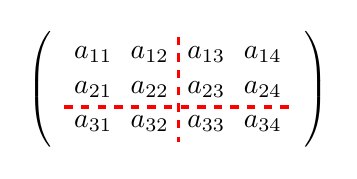
\begin{tikzpicture}
    \matrix(A) [matrix of math nodes,nodes in empty cells,ampersand replacement=\&,left delimiter=(,right delimiter=)] {
      a_{11} \& a_{12} \& a_{13}  \& a_{14} \\
      a_{21} \& a_{22} \& a_{23}  \& a_{24} \\
      a_{31} \& a_{32} \& a_{33}  \& a_{34} \\
    };
    \draw[red, dashed, very thick] (A-1-2.north east) -- (A-3-2.south east) (A-2-1.south west) -- (A-2-4.south east);;
  \end{tikzpicture}
    
  \end{center}
  记为
  $$
  \left(
  \begin{array}{cc}
    \A_{11} &  \A_{12}\\
    \A_{21} &  \A_{22}
  \end{array}
  \right)
  $$
  其中
  $$
  \begin{array}{ll}
  \A_{11} = 
  \left(
  \begin{array}{cc}
    a_{11} &  a_{12}\\
    a_{21} &  a_{22}
  \end{array}
  \right),  &
  \A_{12} = 
  \left(
  \begin{array}{cc}
    a_{13} &  a_{14}\\
    a_{23} &  a_{24}
  \end{array}
  \right)\\ [0.3cm]
  \A_{21} = 
  \left(
  \begin{array}{cc}
    a_{31} &  a_{32}
  \end{array}
  \right) , &
  \A_{22} = 
  \left(
  \begin{array}{cc}
    a_{33} &  a_{34}
  \end{array}
  \right)    
  \end{array}
  $$
    
  \end{footnotesize}
  
\end{frame}


\begin{frame}
  \begin{footnotesize}
    \begin{block}{矩阵的按行分块}
      $$
      \A = \left(
      \begin{array}{cccc}
        a_{11} & a_{12} & \cd & a_{1n}\\
        a_{21} & a_{22} & \cd & a_{2n}\\
        \vd & \vd & & \vd \\
        a_{m1} & a_{m2} & \cd & a_{mn}
      \end{array}
      \right)
      = \left(
      \begin{array}{c}
        \abd_1\\
        \abd_2\\
        \vd \\
        \abd_m
      \end{array}
      \right)
      $$
      其中
      $$
      \abd_i = (a_{i1}, ~a_{i2}, ~\cd, ~a_{in})
      $$
    \end{block}
    
  \end{footnotesize}
   
\end{frame}


\begin{frame}
  \begin{footnotesize}
    \begin{block}{矩阵的按列分块}
      $$
      \B = \left(
      \begin{array}{cccc}
        b_{11} & b_{12} & \cd & b_{1s}\\
        b_{21} & b_{22} & \cd & b_{2s}\\
        \vd & \vd & & \vd \\
        b_{n1} & b_{n2} & \cd & b_{ns}
      \end{array}
      \right)
      = \left(
      \begin{array}{c}
        \bb_1, ~ \bb_2, ~ \cd, \bb_s
      \end{array}
      \right)
      $$
      其中
      $$
      \bb_j = \left(
      \begin{array}{c}
        b_{1j}\\
        b_{2j}\\
        \vd\\
        b_{nj}
      \end{array}
      \right)
      $$
    \end{block}
      
  \end{footnotesize}
\end{frame}




\begin{frame}
  \begin{footnotesize}
  当$n$阶矩阵$\A$中非零元素都集中在主对角线附近,有时可分块成如下\red{对角块矩阵}
  $$
  \A = \left(
  \begin{array}{cccc}
    \A_1 & & &\\
    &\A_2&&\\
    &&\dd&\\
    &&&\A_m
  \end{array}
  \right)
  $$
  其中$\A_i$为$r_i$阶方阵($i=1,2,\cd,m$),且
  $$
  \sum_{i=1}^m r_i = n.
  $$
    
  \end{footnotesize}
\end{frame}

\begin{frame}
    \begin{center}
      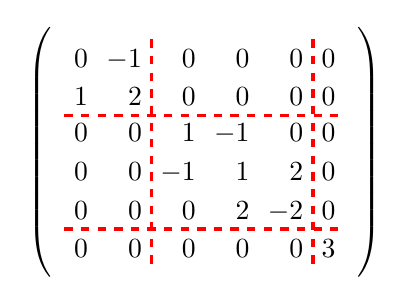
\begin{tikzpicture}       
        [column 1/.style={anchor=base east},
          column 2/.style={anchor=base east},
          column 3/.style={anchor=base east},
          column 4/.style={anchor=base east},
          column 5/.style={anchor=base east},
          column 6/.style={anchor=base east}]
        \matrix(A) [matrix of math nodes,nodes in empty cells,ampersand replacement=\&,left delimiter=(,right delimiter=)] {
          0 \& -1 \& 0 \& 0 \& 0 \& 0\\
          1 \&  2 \& 0 \& 0 \& 0 \& 0\\
          0 \&  0 \& 1 \&-1 \& 0 \& 0\\
          0 \&  0 \&-1 \& 1 \& 2 \& 0\\
          0 \&  0 \& 0 \& 2 \&-2 \& 0\\
          0 \&  0 \& 0 \& 0 \& 0 \& 3\\
        };
        \draw[red, dashed, very thick] 
        (A-1-2.north east) -- (A-6-2.south east)
        (A-1-5.north east) -- (A-6-5.south east) 
        (A-2-1.south west) -- (A-2-6.south east)
        (A-5-1.south west) -- (A-5-6.south east);

      \end{tikzpicture}
    \end{center}
    
\end{frame}

\begin{frame}
  \begin{footnotesize}
  \begin{block}{分块矩阵的加法}
    设$\A, \B$为同型矩阵,采用相同的分块法,有
    $$
    \A = \left(
    \begin{array}{ccc}
      \A_{11} & \cd & \A_{1r} \\
      \vd   &     & \vd   \\
      \A_{s1} & \cd & \A_{sr}
    \end{array}
    \right), \ \ 
    \B = \left(
    \begin{array}{ccc}
      \B_{11} & \cd & \B_{1r} \\
      \vd   &     & \vd   \\
      \B_{s1} & \cd & \B_{sr}
    \end{array}
    \right),
    $$
    其中$\A_{ij}$与$\B_{ij}$为同型矩阵,则
    $$
    A = \left(
    \begin{array}{ccc}
      \A_{11} + \B_{11}  & \cd & \A_{1r} + \B_{1r} \\
      \vd   &     & \vd   \\
      \A_{s1} + \B_{s1}  & \cd & \A_{sr} + \B_{sr}
    \end{array}
    \right).
    $$
  \end{block}
    
  \end{footnotesize}

\end{frame}

\begin{frame}

    \begin{block}{分块矩阵的数乘}
            $$
      \lambda \A = \left(
      \begin{array}{ccc}
        \lambda \A_{11} & \cd & \lambda \A_{1r} \\
        \vd   &     & \vd   \\
        \lambda \A_{s1} & \cd & \lambda \A_{sr}
      \end{array}
      \right)
      $$    
    \end{block}

\end{frame}


\begin{frame}
  \begin{footnotesize}
    \begin{block}{分块矩阵的乘法}
            设$\A$为$m\times n$矩阵, $\B$为$n \times s$矩阵,
      $$
      \A = \left(
      \begin{array}{ccc}
        \A_{11} & \cd & \A_{1s} \\
        \vd   &     & \vd   \\
        \A_{r1} & \cd & \A_{rs}
      \end{array}
      \right), \ \ 
      \B = \left(
      \begin{array}{ccc}
        \B_{11} & \cd & \B_{1t} \\
        \vd   &     & \vd   \\
        \B_{s1} & \cd & \B_{st}
      \end{array}
      \right),
      $$
      其中$\A_{i1}, \A_{i2}, \cd, A_{is}$的列数分别等于$\B_{1j}, \B_{2j}, \cd, \B_{sj}$的行数,则
      $$
      \A \B = \left(
      \begin{array}{ccc}
        \C_{11}   & \cd & \C_{1t}  \\
        \vd   &     & \vd   \\
        \C_{r1}   & \cd & \C_{rt}
      \end{array}
      \right),
      $$
      其中
      $$
      \C_{ij} = \sum_{k=1}^s \A_{ik} \B_{kj}.
      $$
    \end{block}
    
  \end{footnotesize}

\end{frame}

\begin{frame}
  \begin{footnotesize}
    \begin{exampleblock}{例1}
      用分块矩阵的乘法计算$\A\B$,其中
      $$
      \A = \left(
      \begin{array}{rrrrr}
        1&0&0&0&0\\
        0&1&0&0&0\\
        -1&2&1&0&0\\
        1&1&0&1&0\\
        -2&0&0&0&1
      \end{array}
      \right), \quad
      \B = \left(
      \begin{array}{rrrrr}
        3&2&0&1&0\\
        1&3&0&0&1\\
        -1&0&0&0&0\\
        0&-1&0&0&0\\
        0&0&-1&0&0
      \end{array}
      \right)
      $$
    \end{exampleblock}
    \pause 
    \jiename
    \begin{center}
      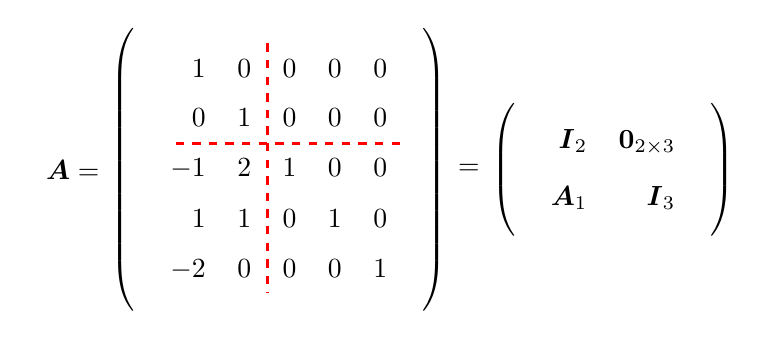
\begin{tikzpicture}       
        [column 1/.style={anchor=base east},
          column 2/.style={anchor=base east},
          column 3/.style={anchor=base east},
          column 4/.style={anchor=base east},
          column 5/.style={anchor=base east}]
        \matrix(A1) [matrix of math nodes]{
          \A = \\
        };
        \matrix(A2) [right=.1in of A1,matrix of math nodes,nodes in empty cells,inner sep=0.2cm,ampersand replacement=\&,left delimiter=(,right delimiter=)] {
          1 \& 0 \& 0 \& 0 \& 0 \\
          0 \& 1 \& 0 \& 0 \& 0 \\
         -1 \& 2 \& 1 \& 0 \& 0 \\
          1 \& 1 \& 0 \& 1 \& 0 \\
         -2 \& 0 \& 0 \& 0 \& 1 \\
        };
        \draw[red, dashed, very thick] 
        (A2-1-2.north east) -- (A2-5-2.south east)
        (A2-2-1.south west) -- (A2-2-5.south east);
        \matrix(A3) [right=.1in of A2,matrix of math nodes]{
          = \\
        };
        \matrix(A4) [right=.1in of A3,matrix of math nodes,nodes in empty cells,inner sep=0.2cm,ampersand replacement=\&,left delimiter=(,right delimiter=)] {
          \II_2 \& \zero_{2\times 3} \\
          \A_1 \& \II_3\\
        };
      \end{tikzpicture}
    \end{center}
    
  \end{footnotesize}
\end{frame}


\begin{frame}
  \begin{footnotesize}
        \begin{center}
      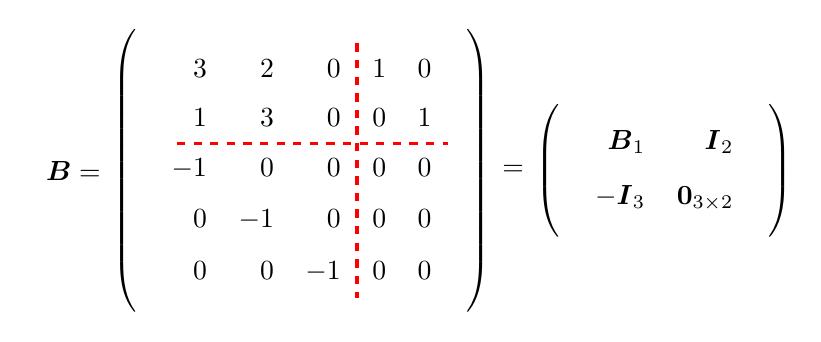
\begin{tikzpicture}       
        [column 1/.style={anchor=base east},
          column 2/.style={anchor=base east},
          column 3/.style={anchor=base east},
          column 4/.style={anchor=base east},
          column 5/.style={anchor=base east}]
        \matrix(A1) [matrix of math nodes]{
          \B = \\
        };
        \matrix(A2) [right=.1in of A1,matrix of math nodes,nodes in empty cells,inner sep=0.2cm,ampersand replacement=\&,left delimiter=(,right delimiter=)] {
          3\&2\&0\&1\&0\\
          1\&3\&0\&0\&1\\
          -1\&0\&0\&0\&0\\
          0\&-1\&0\&0\&0\\
          0\&0\&-1\&0\&0\\
        };
        \draw[red, dashed, very thick] 
        (A2-1-3.north east) -- (A2-5-3.south east)
        (A2-2-1.south west) -- (A2-2-5.south east);
        \matrix(A3) [right=.1in of A2,matrix of math nodes]{
          = \\
        };
        \matrix(A4) [right=.1in of A3,matrix of math nodes,nodes in empty cells,inner sep=0.2cm,ampersand replacement=\&,left delimiter=(,right delimiter=)] {
          \B_1 \& \II_2 \\
          -\II_3 \& \zero_{3\times 2}\\
        };
      \end{tikzpicture}
    \end{center}
        \pause 
        则
        $$
        \A\B = \left(
        \begin{array}{cc}
          \II_2 & \zero\\
          \A_1 & \II_3
        \end{array}
        \right)\left(
        \begin{array}{cc}
          \B_1 & \II_2\\
          -\II_3 & \zero
        \end{array}
        \right) = \left(
        \begin{array}{cc}
          \B_1 & \II_2\\
          \A_1\B_1-\II_3 & \A_1
        \end{array}
        \right)
        $$
        \pause 
        其中
        $$
        \A_1\B_1-\II_3 = \left(
        \begin{array}{rr}
          -1&2\\
          1&1\\
          -2&0
        \end{array}
        \right)\left(
        \begin{array}{rrr}
          3&2&0\\
          1&3&0
        \end{array}
        \right)-\left(
        \begin{array}{ccc}
          1&0&0\\
          0&1&0\\
          0&0&1
        \end{array}
        \right)=\left(
        \begin{array}{rrr}
          -2&4&0\\
          4&4&0\\
          -6&-4&-1
        \end{array}
        \right)
        $$
  \end{footnotesize}
\end{frame}


\begin{frame}
  \begin{footnotesize}
    \begin{exampleblock}{例2}
      设$\A$为$m\times n$矩阵,$\B$为$n\times s$矩阵,$\B$按列分块成$1\times s$分块矩阵,
      将$\A$看成$1\times 1$分块矩阵,则
      $$
      \A\B=\A(\bb_1,\bb_2,\cd,\bb_s)=(\A\bb_1,\A\bb_2,\cd,\A\bb_s)      
      $$
      若已知$\A\B=0$,则显然
      $$
      \A\bb_j=0, \quad j=1,2,\cd,s.
      $$
      因此,$\B$的每一列$\bb_j$都是线性方程组$\A\xx=0$的解。
    \end{exampleblock}    
  \end{footnotesize}
\end{frame}


\begin{frame}
  \begin{footnotesize}
    \begin{exampleblock}{例3}
      设$\A^T\A=\zero$,证明$\A=\zero$.
    \end{exampleblock}
    \pause
    \proofname
    设$\A=(a_{ij})_{m\times n}$,把$\A$用列向量表示为$\A=(\abd_1, ~\abd_2,~\cd,~\abd_n)$,则
    $$
    \A^T\A = \left(
    \begin{array}{c}
      \abd_1^T\\
      \abd_2^T\\
      \cd \\
      \abd_n^T
    \end{array}
    \right) (\abd_1, ~\abd_2,~\cd,~\abd_n) = \left(
    \begin{array}{cccc}
      \abd_1^T\abd_1 & \abd_1^T\abd_2 & \cd & \abd_1^T\abd_n\\
      \abd_2^T\abd_1 & \abd_2^T\abd_2 & \cd & \abd_2^T\abd_n\\
      \vd & \vd & & \vd \\
      \abd_n^T\abd_1 & \abd_n^T\abd_2 & \cd & \abd_n^T\abd_n
    \end{array}
    \right)
    $$
    \pause 
    因为$\A^T\A=\zero$,故
    $$
    \abd_i^T \abd_j = 0, \quad i,j=1,2,\cd,n.
    $$
    \pause
    特别地,有
    $$
    \abd_j^T \abd_j = 0, \quad j=1,2,\cd,n,
    $$\pause
    即
    $$
    a_{1j}^2+a_{2j}^2+\cd+a_{mj}^2=0 \pause ~\Rightarrow~ a_{1j}=a_{2j}=\cd=a_{mj}=0 \pause~\Rightarrow~ \A = \zero.
    $$
  \end{footnotesize}
\end{frame}

\begin{frame}
  \begin{footnotesize}
  \begin{exampleblock}{例4}
    若$n$阶矩阵$\C,\D$可以分块成同型对角块矩阵,即
    $$
    \C = \left(
    \begin{array}{cccc}
      \C_1&&&\\
      &\C_2&&\\
      &&\cd&\\
      &&&\C_m
    \end{array}
    \right),\quad
    \D = \left(
    \begin{array}{cccc}
      \D_1&&&\\
      &\D_2&&\\
      &&\cd&\\
      &&&\D_m
    \end{array}
    \right)
    $$
    其中$\C_i$和$\D_i$为同阶方阵($i=1,2,\cd,m$),则
    $$
    \C\D = \left(
    \begin{array}{cccc}
      \C_1\D_1&&&\\
      &\C_2\D_2&&\\
      &&\cd&\\
      &&&\C_m\D_m
    \end{array}
    \right)
    $$
  \end{exampleblock}
    
  \end{footnotesize}
\end{frame}


\begin{frame}
  \begin{footnotesize}
    \begin{exampleblock}{例5}
      证明:若方阵$\A$为可逆的上三角阵,则$\A^{-1}$也为上三角阵。
    \end{exampleblock}
    \pause
    \proofname
    对阶数$n$用数学归纳法。
    \begin{itemize}
    \item[1] 当$n=1$时,$(a)^{-1}=(\frac1a)$,结论成立。\pause 
    \item[2] 假设命题对$n-1$阶可逆上三角矩阵成立,考虑$n$阶情况,设
      \begin{center}
        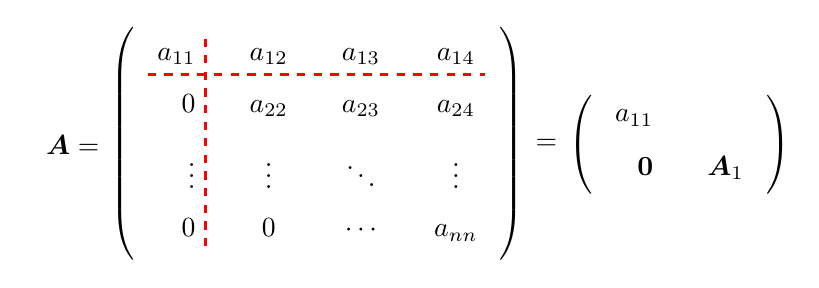
\begin{tikzpicture} [column 1/.style={anchor=base east}]
          \matrix (M) [matrix of math nodes]  { 
            \A = \\
          };
          \matrix(MM) [right=.1in of M, matrix of math nodes,nodes in empty cells,
            column sep=3ex,row sep=1ex,ampersand replacement=\&,left delimiter=(,right delimiter=)] {
            a_{11} \& a_{12} \& a_{13}  \& a_{14} \\
            0    \& a_{22} \& a_{23}  \& a_{24} \\
            \vd  \& \vd   \& \dd  \& \vd \\
            0    \& 0     \& \cd  \& a_{nn} \\
          };
                
          \draw[red, dashed, very thick]
          (MM-1-1.north east) -- (MM-4-1.south east)
          (MM-1-1.south west) -- (MM-1-4.south east);

          \matrix (MMM) [right=.1in of MM,matrix of math nodes]  { 
            = \\
          };
          \matrix(MMMM) [right=.1in of MMM, matrix of math nodes,nodes in empty cells,
            column sep=3ex,row sep=1ex,ampersand replacement=\&,left delimiter=(,right delimiter=)] {
            a_{11} \& \alphabd\\
            \zero \& \A_1\\
          };
        \end{tikzpicture}        
      \end{center}
      其中$\A_1$为$n-1$阶可逆上三角阵。
    \end{itemize}
  \end{footnotesize}
\end{frame}


\begin{frame}
  \begin{footnotesize}
    设$\A$的逆阵为
    $$
    \B = \left(
    \begin{array}{cc}
      b_{11} & \betabd\\
      \gammabd & \B_1 
    \end{array}    
    \right), \pause 
    \quad \betabd = \left(
    \begin{array}{c}
      b_{12}\\
      \vd \\
      b_{1n}
    \end{array}
    \right)^T,
    \quad \gammabd = \left(
    \begin{array}{c}
      b_{21}\\
      \vd \\
      b_{n1}
    \end{array}
    \right), \quad
    \B_1 = \left(
    \begin{array}{ccc}
      b_{22} & \cd & b_{2n}\\
      \vd   & \dd & \vd \\
      b_{n2} & \cd & b_{nn}
    \end{array}
    \right)
    $$
    \pause
    则
    $$
    \A\B = \left(
    \begin{array}{cc}
      a_{11} & \alphabd \\
      \zero & \A_1
    \end{array}
    \right)\left(
    \begin{array}{cc}
      b_{11} & \betabd \\
      \gammabd & \B_1
    \end{array}
    \right) = \left(
    \begin{array}{cc}
      a_{11}b_{11}+\alphabd\gammabd & a_{11}\betabd+\alphabd \B_1\\
      \A_1\gammabd & \A_1\B_1
    \end{array}
    \right) \pause \red{
      = \left(
      \begin{array}{cc}
        1 & \zero \\
        \zero & \II_{n-1}
      \end{array}
      \right)
      }
    $$
    \pause
    于是
    $$
    \begin{array}{l}
      \A_1 \gammabd = \zero ~ \Rightarrow ~ \gammabd=\zero, \\[0.2cm]
      \A_1\B_1 = \II_1 ~\Rightarrow~ \B_1=\A_1^{-1}.
    \end{array}
    $$
    由归纳假设,$\B_1$为$n-1$阶上三角矩阵,因此
    $$
    \A^{-1} = \B = \left(
    \begin{array}{cc}
      b_{11} & \betabd\\
      \zero & \B_1 
    \end{array}    
    \right)
    $$
    为上三角矩阵。
  \end{footnotesize}
\end{frame}

\begin{frame}
  \begin{footnotesize}
    \begin{block}{分块矩阵的转置}
      分块矩阵$\A=(\A_{kl})_{s\times t}$的转置矩阵为
      $$
      \A^T = (\B_{lk})_{t\times s},
      $$
      其中$\B_{lk}=\A_{kl}$.
    \end{block}
    \pause
    \begin{exampleblock}{例}
      $$
      \A = \left(
      \begin{array}{ccc}
        \A_{11} & \A_{12} & \A_{13}\\
        \A_{21} & \A_{22} & \A_{23}
      \end{array}
      \right) ~\Rightarrow~
      \A = \left(
      \begin{array}{cc}
        \A_{11}^T & \A_{21}^T \\[0.2cm]
        \A_{12}^T & \A_{22}^T \\[0.2cm]
        \A_{13}^T & \A_{23}^T
      \end{array}
      \right)
      $$
      \pause
      $$
      \B \xlongequal[]{\mbox{按行分块}} \left(
      \begin{array}{c}
        \bb_1\\
        \bb_2\\
        \vd\\
        \bb_m
      \end{array}
      \right) ~\Rightarrow~
      \B^T = \left(
      \begin{array}{cccc}
        \bb_1^T & \bb_2^T & \cd & \bb_m^T
      \end{array}
      \right)
      $$
    \end{exampleblock}
  \end{footnotesize}
\end{frame}


\begin{frame}
  \begin{footnotesize}
    \begin{block}{可逆分块矩阵的逆矩阵}
      对角块矩阵(准对角矩阵)
      $$
      \A = \left(
      \begin{array}{cccc}
        \A_1&&&\\
        &\A_2&&\\
        &&\dd&\\
        &&&\A_m
      \end{array}
      \right)
      $$
      的行列式为$|\A|=|\A_1||\A_2|\cd|\A_m|$,因此,$\A$可逆的充分必要条件为
      $$
      |\A_i|\ne 0, \quad i=1,2,\cd, m.
      $$
      \pause
      其逆矩阵为
      $$
      \A^{-1} = \left(
      \begin{array}{cccc}
        \A_1^{-1}&&&\\
        &\A_2^{-1}&&\\
        &&\dd&\\
        &&&\A_m^{-1}
      \end{array}
      \right)
      $$
    \end{block}
  \end{footnotesize}
\end{frame}


\begin{frame}
  \begin{itemize}
  \item   用分块矩阵求逆矩阵,可将高阶矩阵的求逆转化为低阶矩阵的求逆。\\[0.1in]
  \item   一个$2\times 2$的分块矩阵求逆,可以根据逆矩阵的定义,用解矩阵方程的方法解得。
  \end{itemize}
\end{frame}


\begin{frame}
  \begin{footnotesize}
    \begin{exampleblock}{例6}
      设$\A=\left(
      \begin{array}{cc}
        \B&\zero\\
        \C&\D
      \end{array}
      \right)$,其中$\B,\D$皆为可逆矩阵,证明$\A$可逆并求$\A^{-1}$.
    \end{exampleblock}
    \pause 
    \jiename
    因$|\A|=|\B||\D|\ne 0$,故$\A$可逆。设$\A^{-1}=\left(
    \begin{array}{cc}
      \X&\Y\\
      \Z&\T
    \end{array}
    \right)$,则
    $$
    \left(
    \begin{array}{cc}
      \B&\zero\\
      \C&\D
    \end{array}
    \right) \left(
    \begin{array}{cc}
      \X&\Y\\
      \Z&\T
    \end{array}
    \right)=\left(
    \begin{array}{cc}
      \B\X&\B\Y\\
      \C\X+\D\Z&\C\Y+\D\T
    \end{array}
    \right) = \left(
    \begin{array}{cc}
      \II & \zero\\
      \zero & \II
    \end{array}
    \right)
    $$
    \pause
    由此可知
    $$
    \begin{array}{ll}
      \B\X = \II   & \Rightarrow ~ \X = \B^{-1}\\[0.2cm]
      \B\Y = \zero & \Rightarrow ~ \Y = \zero\\[0.2cm]
      \C\X+\D\Z = \zero & \Rightarrow ~ \Z = -\D^{-1}\C\B^{-1}\\[0.2cm]
      \C\Y+\D\T = \II & \Rightarrow ~ \T = \D^{-1}
    \end{array}
    $$
    \pause 
    故
    $$
    \A^{-1} = \left(
    \begin{array}{cc}
      \B^{-1} & \zero\\
      -\D^{-1}\C\B^{-1} & \D^{-1}
    \end{array}
    \right).
    $$
  \end{footnotesize}
\end{frame}


\begin{frame}
  \begin{footnotesize}
    \begin{exampleblock}{分块矩阵的初等变换与分块初等矩阵}
      对于分块矩阵
      $$
      \A = \left(
      \begin{array}{cc}
        \A_{11} & \A_{12}\\
        \A_{21} & \A_{22}
      \end{array}
      \right)
      $$
      同样可以定义它的3类初等行变换与列变换,并相应地定义3类分块矩阵:
      \begin{itemize}
      \item[(i)] 分块倍乘矩阵($\C_1,\C_2$为可逆阵)
        $$
        \left(
        \begin{array}{cc}
          \C_1 & \zero\\
          \zero & \II_n
        \end{array}
        \right) ~~\mbox{或}~~
        \left(
        \begin{array}{cc}
          \II_m & \zero\\
          \zero & \C_2
        \end{array}
        \right)
        $$
      \item[(ii)] 分块倍加矩阵
        $$
        \left(
        \begin{array}{cc}
          \II_m & \zero\\
          \C_3 & \II_n
        \end{array}
        \right) ~~\mbox{或}~~
        \left(
        \begin{array}{cc}
          \II_m & \C_4\\
          \zero & \II_n
        \end{array}
        \right)
        $$
      \item[(iii)] 分块对换矩阵
        $$
        \left(
        \begin{array}{cc}
          \zero & \II_n\\
          \II_m & \zero
        \end{array}
        \right)
        $$
      \end{itemize}
    \end{exampleblock}
  \end{footnotesize}
\end{frame}


\begin{frame}
  \begin{footnotesize}
    \begin{exampleblock}{例7}
      设$n$阶矩阵$\A$分块表示为
      $$
      \A = \left(
      \begin{array}{cc}
        \A_{11} & \A_{12}\\
        \A_{21} & \A_{22}
      \end{array}
      \right)
      $$
      其中$\A_{11},\A_{22}$为方阵,且$\A$与$\A_{11}$可逆。证明:$\A_{22}-\A_{21}\A_{11}^{-1}\A_{12}$可逆,并求$\A^{-1}$。
    \end{exampleblock}
    \pause
    \jiename
    构造分块倍加矩阵
    $$
    \PP_1 = \left(
    \begin{array}{cc}
      \II_1 & \zero\\
      -\A_{21}\A_{11}^{-1} & \II_2
    \end{array}
    \right)
    $$
    则$$
    \PP_1\A = \left(
    \begin{array}{cc}
      \A_{11} & \A_{12} \\
      \zero & \A_{22}-\A_{21}\A_{11}^{-1}\A_{12}
    \end{array}
    \right)
    $$
    两边同时取行列式可知
    $$
    |\A| = |\PP_1\A| = |\A_{11}|\cdot |\A_{22}-\A_{21}\A_{11}^{-1}\A_{12}|
    $$
    故$\A_{22}-\A_{21}\A_{11}^{-1}\A_{12}$可逆。
  \end{footnotesize}
\end{frame}

\begin{frame}
  \begin{footnotesize}
    $$
    \PP_1\A = \left(
    \begin{array}{cc}
      \A_{11} & \A_{12} \\
      \zero & \A_{22}-\A_{21}\A_{11}^{-1}\A_{12}
    \end{array}
    \right)\xlongequal[]{\red{\disp \QQ=\A_{22}-\A_{21}\A_{11}^{-1}\A_{12}}}
    \left(
    \begin{array}{cc}
      \A_{11} & \A_{12} \\
      \zero & \QQ
    \end{array}
    \right)
    $$ \pause
    构造分块倍加矩阵
    $$
    \PP_2 = \left(
    \begin{array}{cc}
      \II_1 & -\A_{12}\QQ^{-1}\\
      \zero & \II_2
    \end{array}
    \right)
    $$ \pause
    则
    $$
    \PP_2\PP_1\A = \left(
    \begin{array}{cc}
      \A_{11} & \zero\\
      \zero & \QQ
    \end{array}
    \right)
    $$ \pause
    于是
    $$
    \begin{array}{rl}
      \A^{-1} & \pause= \left(
      \begin{array}{cc}
        \A_{11}^{-1} & \zero\\
        \zero & \QQ^{-1}
      \end{array}
      \right)\left(
      \begin{array}{cc}
        \II_1 & -\A_{12}\QQ^{-1}\\
        \zero & \II_2
      \end{array}
      \right)\left(
      \begin{array}{cc}
        \II_1 & \zero\\[0.2cm]
        -\A_{21}\A_{11}^{-1} & \II_2
      \end{array}
      \right) \\[0.3in]
      & \pause= \left(
      \begin{array}{cc}
        \A_{11}^{-1} & \zero\\[0.2cm]
        \zero & \QQ^{-1}
      \end{array}
      \right)\left(
      \begin{array}{cc}
        \II_1+ \A_{12}\QQ^{-1}\A_{21}\A_{11}^{-1}& -\A_{12}\QQ^{-1}\\[0.2cm]
        -\A_{21}\A_{11}^{-1} & \II_2
      \end{array}
      \right)\\[0.3in]
      & \pause= \left(
      \begin{array}{cc}
        \A_{11}^{-1}+ \A_{11}^{-1}\A_{12}\QQ^{-1}\A_{21}\A_{11}^{-1}& -\A_{11}^{-1}\A_{12}\QQ^{-1}\\[0.2cm]
        -\QQ^{-1}\A_{21}\A_{11}^{-1} & \QQ^{-1}
      \end{array}
      \right)
    \end{array}
    $$
  \end{footnotesize}
\end{frame}



\begin{frame}
  \begin{footnotesize}
    \begin{exampleblock}{例8}
      设$\QQ=\left(
      \begin{array}{cc}
        \A&\B\\
        \C&\D
      \end{array}
      \right)$,且$\A$可逆,证明:
      $$
      |\QQ| = |\A| \cdot |\D-\C\A^{-1}\B|
      $$
    \end{exampleblock}
    \pause
    \jiename
    构造分块倍加矩阵
    $$
    \PP_1 = \left(
    \begin{array}{cc}
      \II_1 & \zero\\
      -\C\A^{-1} & \II_2
    \end{array}
    \right)
    $$\pause 
    则
    $$
    \PP_1 \QQ = \left(
    \begin{array}{cc}
      \A & \B\\
      \zero & \D-\C\A^{-1}\B
    \end{array}
    \right)
    $$
    \pause
    两边同时取行列式得
    $$
    |\QQ| = |\PP_1\QQ| = |\A|\cdot |\D-\C\A^{-1}\B|.
    $$
  \end{footnotesize}
\end{frame}

\begin{frame}
  \begin{footnotesize}
    \begin{exampleblock}{例9}
      设$\A$与$\B$均为$n$阶分块矩阵,证明
      $$
      \left|
      \begin{array}{cc}
        \A&\B\\
        \B&\A
      \end{array}
      \right| = |\A+\B|~|\A-\B|
      $$
    \end{exampleblock}
    \pause
    \jiename
    将分块矩阵$
    \PP = 
    \left(
    \begin{array}{cc}
      \A&\B\\
      \B&\A
    \end{array}
    \right)$的第一行加到第二行,得
    $$
    \left(
    \begin{array}{cc}
      \II & \zero\\
      \II & \II
    \end{array}
    \right) \left(
    \begin{array}{cc}
      \A&\B\\
      \B&\A
    \end{array}
    \right) = \left(
    \begin{array}{cc}
      \A&\B\\
      \A+\B&\A+\B
    \end{array}
    \right)
    $$\pause
    再将第一列减去第二列,得
    $$
    \left(
    \begin{array}{cc}
      \A&\B\\
      \A+\B&\A+\B
    \end{array}
    \right) \left(
    \begin{array}{cc}
      \II&\zero\\
      -\II&\II
    \end{array}
    \right) = \left(
    \begin{array}{cc}
      \A-\B & \B\\
      \zero & \A+\B
    \end{array}
    \right)
    $$\pause
    总之有
    $$
    \left(
    \begin{array}{cc}
      \II & \zero\\
      \II & \II
    \end{array}
    \right) \left(
    \begin{array}{cc}
      \A&\B\\
      \B&\A
    \end{array}
    \right) 
    \left(
    \begin{array}{cc}
      \II&\zero\\
      -\II&\II
    \end{array}
    \right) = \left(
    \begin{array}{cc}
      \A-\B & \B\\
      \zero & \A+\B
    \end{array}
    \right)
    $$
    两边同时取行列式即得结论。
  \end{footnotesize}
\end{frame}

%  \section{习题}

\begin{frame}
  \begin{footnotesize}
    \begin{exampleblock}{28}
      求与$\A=\left(
      \begin{array}{rrr}
        1&0&0\\
        0&1&2\\
        0&1&-2
      \end{array}
      \right)$可交换的全体三阶矩阵。
    \end{exampleblock}
  \end{footnotesize}
\end{frame}



\begin{frame}
  \begin{footnotesize}
    \begin{exampleblock}{29}
      已知$\A$是对角元互不相等的$n$阶对角矩阵,即
      $$
      \A=\left(
      \begin{array}{cccc}
        a_1&&&\\
        &a_2&&\\
        &&\dd&\\
        &&&a_n
      \end{array}
      \right)
      $$
      当$i\ne j$时,$a_i\ne a_j$。证明:与$\A$可交换的矩阵必是对角矩阵。
    \end{exampleblock}
    \pause\proofname
    设与$\A$可交换的矩阵为$\B=\left(
    \begin{array}{rrrr}
      b_{11}&b_{12}&\cd&b_{1n}\\
      b_{21}&b_{22}&\cd&b_{2n}\\
      \vd&\vd&\dd&\vd\\
      b_{n1}&b_{n2}&\cd&b_{nn}
    \end{array}
    \right)$
    由$\A\B=\B\A$,即
    $$
    \left(
    \begin{array}{rrrr}
      a_1b_{11}&a_1b_{12}&\cd&a_1b_{1n}\\
      a_2b_{21}&a_2b_{22}&\cd&a_2b_{2n}\\
      \vd&\vd&\dd&\vd\\
      a_nb_{n1}&a_nb_{n2}&\cd&a_nb_{nn}
    \end{array}
    \right)=\left(
    \begin{array}{rrrr}
      a_1b_{11}&a_2b_{12}&\cd&a_nb_{1n}\\
      a_1b_{21}&a_2b_{22}&\cd&a_nb_{2n}\\
      \vd&\vd&\dd&\vd\\
      a_1b_{n1}&a_2b_{n2}&\cd&a_nb_{nn}
    \end{array}
    \right)
    $$
  \end{footnotesize}
\end{frame}

\begin{frame}
  \begin{footnotesize}
    亦即
    $$
    \left(
    \begin{array}{rrrr}
      0&(a_1-a_2)b_{12}&\cd&(a_1-a_n)b_{1n}\\
      (a_2-a_1)b_{21}&0&\cd&(a_2-a_n)b_{2n}\\
      \vd&\vd&\dd&\vd\\
      (a_n-a_1)b_{n1}&(a_n-a_2)b_{n2}&\cd&0
    \end{array}
    \right)=\zero
    $$
    因为$a_i\ne a_j(i\ne j)$,故
    $$
    b_{ij}=0, \quad i\ne j
    $$
  \end{footnotesize}
\end{frame}

\begin{frame}
  \begin{footnotesize}
    \begin{exampleblock}{30}
      证明:两个$n$阶下三角矩阵的乘积仍是下三角矩阵。
    \end{exampleblock}
  \end{footnotesize}
\end{frame}



\begin{frame}
  \begin{footnotesize}
    \begin{exampleblock}{31}
      证明:若$\A$是对角元全为零的上三角矩阵,则$\A^2$也是主对角元全为零的上三角矩阵。
    \end{exampleblock}
  \end{footnotesize}
\end{frame}



\begin{frame}
  \begin{footnotesize}
    \begin{exampleblock}{32}
      证明:对角元全为1的上三角矩阵的乘积,仍是主对角元全为1的上三角矩阵。
    \end{exampleblock}
  \end{footnotesize}
\end{frame}


\begin{frame}
  \begin{footnotesize}
    \begin{exampleblock}{33}
      设$$\A=\left(
      \begin{array}{rrr}
        5&-2&1\\
        3&4&-1
      \end{array}
      \right),~~\B=\left(
      \begin{array}{rrr}
        -3&2&0\\
        -2&0&1
      \end{array}
      \right),$$
      计算$\A\B^T,~\B^T\A,~\A^T\A,~\B\B^T+\A\B^T$。
    \end{exampleblock}
  \end{footnotesize}
\end{frame}



\begin{frame}
  \begin{footnotesize}
    \begin{exampleblock}{34}
      证明:$(\A_1\A_2\cd\A_k)^T=\A_k^T\cd\A_2^T\A_1^T$。
    \end{exampleblock}
    \pause\proofname
    由$(\A\B)^T=\B^T\A^T$及数学归纳法容易证明。
  \end{footnotesize}
\end{frame}



\begin{frame}
  \begin{footnotesize}
    \begin{exampleblock}{35}
      证明:若$\A$和$\B$都是$n$阶对称矩阵,则$\A+\B,~~\A-2\B$也是对称矩阵。
    \end{exampleblock}
    \pause\proofname
    对称矩阵的线性组合仍是对称矩阵。
  \end{footnotesize}
\end{frame}



\begin{frame}
  \begin{footnotesize}
    \begin{exampleblock}{36}
      对于任意的$n$阶矩阵$\A$,证明:
      \begin{itemize}
      \item[(1)]$\A+\A^T$是对称矩阵,$\A-\A^T$是反对称矩阵。
      \item[(2)]$\A$可表示对称矩阵和反对称矩阵之和。
      \end{itemize}
    \end{exampleblock}
    \pause\proofname
    $$
    \A = \frac{\A+\A^T}2+\frac{\A-\A^T}2
    $$
  \end{footnotesize}
\end{frame}



\begin{frame}
  \begin{footnotesize}
    \begin{exampleblock}{37}
      证明:若$\A$和$\B$都是$n$阶对称矩阵,则$\A\B$是对称矩阵的充要条件是$\A$与$\B$可交换。
    \end{exampleblock}
    \pause\proofname
    \begin{itemize}
    \item[($\Rightarrow$)]
      $$\A\B\mbox{对称}\Rightarrow \A\B=(\A\B)^T=\B^T\A^T=\B\A$$
    \item[($\Leftarrow$)]
      $$\A\B\mbox{可交换}\Rightarrow\A\B=\B\A\Rightarrow (\A\B)^T=\B^T\A^T=\B\A=\A\B$$
    \end{itemize}
  \end{footnotesize}
\end{frame}


\begin{frame}
  \begin{footnotesize}
    \begin{exampleblock}{38}
      设$\A$是实对称矩阵,且$\A^2=\zero$,证明$\A=\zero$.
    \end{exampleblock}
    \pause\proofname
    因为$\A$实对称,故
    $$
    \A^2=\zero \Longleftrightarrow \A^T\A=\zero
    $$
    观察$\A^T\A$的主对角元,
    $$
    \sum_{i=1}^na_{ij}^2=0
    $$
    故
    $$
    a_{ij}=0 \quad \forall i, j.
    $$
  \end{footnotesize}
\end{frame}



\begin{frame}
  \begin{footnotesize}
    \begin{exampleblock}{39}
      已知$\A$是一个$n$阶对称矩阵,$\B$是一个$n$阶反对称矩阵。
      \begin{itemize}
      \item[(1)]问$\A^k,~~\B^k$是否为对称或反对称矩阵?
      \item[(2)]证明:$\A\B+\B\A$是一个反对称矩阵。
      \end{itemize}
    \end{exampleblock}
    \pause\proofname
    \begin{itemize}
    \item[(1)]
      $$
      (\A^k)^T=(\A\A\cd\A)^T=\A^T\cd\A^T\A^T=\A\cd\A\A=\A^k \red{~~\Longrightarrow~~ \A^k\mbox{对称}}
      $$

      $$
      (\B^k)^T=(-\B)\cd(-\B)(-\B)=(-1)^k\B^k \red{~~\Longrightarrow~~
      \left\{
      \begin{array}{ll}
        \B^k\mbox{对称}, & k\mbox{为偶数}\\
        \B^k\mbox{反对称}, & k\mbox{为奇数}
      \end{array}      
      \right.
    }
      $$
    \item[(2)]
      $$
      \begin{array}{rl}
        (\A\B+\B\A)^T&=(\A\B)^T+(\B\A)^T=\B^T\A^T+\A^T\B^T\\[0.05in]
        &=-\B\A-\A\B.
      \end{array}
      $$
    \end{itemize}
  \end{footnotesize}
\end{frame}



\begin{frame}
  \begin{footnotesize}
    \begin{exampleblock}{40(求逆矩阵)}
      \begin{itemize}
      \item[(1)]
        $$
        \left(
        \begin{array}{rr}
          8&-4\\
          -5&3
        \end{array}
        \right)
        $$
      \end{itemize}
    \end{exampleblock}
  \end{footnotesize}
\end{frame}

\begin{frame}
  \begin{footnotesize}
    \begin{exampleblock}{40(求逆矩阵)}
      \begin{itemize}
      \item[(2)]
        $$
        \left(
        \begin{array}{rr}
          \cos\theta&\sin\theta\\
          -\sin\theta&\cos\theta
        \end{array}
        \right)
        $$
      \end{itemize}
    \end{exampleblock}

    $$
    \left(
    \begin{array}{rr}
      \cos\theta&\sin\theta\\
      -\sin\theta&\cos\theta
    \end{array}
    \right)^{-1}=
    \left(
    \begin{array}{rr}
      \cos(-\theta)&\sin(-\theta)\\
      -\sin(-\theta)&\cos(-\theta)
    \end{array}
    \right)=     \left(
    \begin{array}{rr}
      \cos\theta&-\sin\theta\\
      \sin\theta&\cos\theta
    \end{array}
    \right)
    $$
  \end{footnotesize}
\end{frame}


\begin{frame}
  \begin{footnotesize}
    \begin{exampleblock}{40(求逆矩阵)}
      \begin{itemize}
      \item[(3)]
        $$
        \left(
        \begin{array}{rrr}
          1&2&-2\\
          2&1&-2\\
          2&-2&1
        \end{array}
        \right)
        $$
      \end{itemize}
    \end{exampleblock}
  \end{footnotesize}
\end{frame}

\begin{frame}
  \begin{footnotesize}
    \begin{exampleblock}{40(求逆矩阵)}
      \begin{itemize}
      \item[(4)]
        $$
        \left(
        \begin{array}{rrr}
          2&3&-1\\
          1&2&0\\
          -1&2&-2
        \end{array}
        \right)
        $$
      \end{itemize}
    \end{exampleblock}
  \end{footnotesize}
\end{frame}

\begin{frame}
  \begin{footnotesize}
    \begin{exampleblock}{40(求逆矩阵)}
      \begin{itemize}
      \item[(5)]
        $$
        \left(
        \begin{array}{rrr}
          1&0&0\\
          1&1&0\\
          1&1&1
        \end{array}
        \right)
        $$
      \end{itemize}
    \end{exampleblock}
  \end{footnotesize}
\end{frame}

\begin{frame}
  \begin{footnotesize}
    \begin{exampleblock}{40(求逆矩阵)}
      \begin{itemize}
      \item[(6)]
        $$
        \left(
        \begin{array}{rrrr}
          1&1&0&0\\
          0&1&1&0\\
          0&0&1&1\\
          0&0&0&1
        \end{array}
        \right)
        $$
      \end{itemize}
    \end{exampleblock}
  \end{footnotesize}
\end{frame}


\begin{frame}
  \begin{footnotesize}
    \begin{exampleblock}{41(解矩阵方程)}
      \begin{itemize}
      \item[(2)]
        $$
        \left(
        \begin{array}{rrr}
          2&3&-1\\
          1&2&0\\
          -1&2&-2
        \end{array}
        \right)\X=
        \left(
        \begin{array}{rr}
          2&1\\
          -1&0\\
          3&1
        \end{array}
        \right)        
        $$
      \end{itemize}
    \end{exampleblock}
  \end{footnotesize}
\end{frame}

\begin{frame}
  \begin{footnotesize}
    \begin{exampleblock}{41(解矩阵方程)}
      \begin{itemize}
      \item[(3)]
        $$
        \A\left(
        \begin{array}{rrr}
          1&1&1\\
          0&1&1\\
          0&0&1
        \end{array}
        \right)=
        \left(
        \begin{array}{rrr}
          1&-2&1\\
          0&1&-1
        \end{array}
        \right)        
        $$
      \end{itemize}
    \end{exampleblock}
  \end{footnotesize}
\end{frame}


\begin{frame}
  \begin{footnotesize}
    \begin{exampleblock}{42(解线性方程组)}     
      $$
      \left\{
      \begin{array}{rrrcr}
        x_1&+x_2&+x_3&=&1\\
           &2x_2&+2x_3&=&1\\
        x_1&-x_2&&=&2
      \end{array}
      \right.
      $$
    \end{exampleblock}
  \end{footnotesize}
\end{frame}



\begin{frame}
  \begin{footnotesize}
    \begin{exampleblock}{43}
      设$\A,~\B,~\C$为同阶方阵,
      \begin{itemize}
      \item[(1)]问$\A$满足什么条件时,命题\blue{$\A\B=\A\C~\Rightarrow~\B=\C$}成立;\\[0.05in]
      \item[(2)] 问:若$\B\ne\C$时,是否必有$\A\B\ne\A\C$?
      \end{itemize}
    \end{exampleblock}
    
    \begin{itemize}
    \item[(1)]
      当$\A$可逆时,该命题成立。
    \item[(2)]
      不一定。例如,当$\A=\zero$时,不论任何$\B,\C$,总有$\A\B=\A\C$。

    \end{itemize}

  \end{footnotesize}
\end{frame}


\begin{frame}
  \begin{footnotesize}
    \begin{exampleblock}{44}
      设$\A,~\B$都是$n$阶方阵,问:下列命题是否成立?若成立,给出证明;若不成立,举反例说明。
      \begin{itemize}
      \item[(1)]若$\A,\B$皆不可逆,则$\A+\B$也不可逆;
      \item[(2)]若$\A\B$可逆,则$\A,~\B$都可逆;
      \item[(3)]若$\A\B$不可逆,则$\A,~\B$都不可逆;
      \item[(4)]若$\A$可逆,则$k\A$可逆($k$是数)。
      \end{itemize}
    \end{exampleblock}
    \begin{itemize}
    \item[(1)]不成立。\purple{例如,令$\A=\left(
      \begin{array}{cc}
        1&0\\
        0&0
      \end{array}
      \right),~~\B=\left(
      \begin{array}{cc}
        0&0\\
        0&1
      \end{array}
      \right)$皆不可逆,但$\A+\B=\left(
      \begin{array}{cc}
        1&0\\
        0&1
      \end{array}
      \right)$可逆。}
    \item[(2)]成立。$\purple{\A\B\mbox{可逆}\Rightarrow |\A||\B|=|\A\B|\ne 0 \Rightarrow |\A|\ne0\mbox{且}|\B|\ne 0
      \Rightarrow \A,~\B\mbox{都可逆。}}$
    \item[(3)]不成立。\purple{例如,令$\A=\left(
      \begin{array}{cc}
        0&0\\
        0&0
      \end{array}
      \right),~~\B=\left(
      \begin{array}{cc}
        1&0\\
        0&1
      \end{array}
      \right)$,则$\A\B=\zero$不可逆,但$\A$不可逆,但$\B$可逆。}
    \item[(4)]不成立。\purple{$\A\mbox{可逆} \Rightarrow \left\{
      \begin{array}{rl}
        k\A\mbox{可逆},& k\ne 0, \\
        k\A\mbox{不可逆},& k= 0.
      \end{array}
      \right.
      $}
    \end{itemize}

  \end{footnotesize}
\end{frame}



\begin{frame}
  \begin{footnotesize}
    \begin{exampleblock}{45}
      设方阵$\A$满足$\A^2-\A-2\II=\zero$,证明:
      \begin{itemize}
      \item[(1)]$\A$和$\II-\A$都可逆,并求它们的逆;
      \item[(2)]$\A+\II$和$\A-2\II$不同时可逆。
      \end{itemize}
    \end{exampleblock}
  \end{footnotesize}
\end{frame}



\begin{frame}
  \begin{footnotesize}
    \begin{exampleblock}{46}
      设方阵$\A$满足$\A^2-2\A+4\II=\zero$,证明$\A+\II$和$\A-3\II$都可逆,并求它们的逆。
    \end{exampleblock}
  \end{footnotesize}
\end{frame}



\begin{frame}
  \begin{footnotesize}
    \begin{exampleblock}{47}
      试求上(或下)三角矩阵可逆的充要条件,并证明:可逆上(或下)三角矩阵的逆矩阵也是可逆上(或下)三角矩阵。
    \end{exampleblock}
  \end{footnotesize}
\end{frame}



\begin{frame}
  \begin{footnotesize}
    \begin{exampleblock}{28}
      
    \end{exampleblock}
  \end{footnotesize}
\end{frame}


\begin{frame}
  \begin{footnotesize}
    \begin{exampleblock}{28}
      
    \end{exampleblock}
  \end{footnotesize}
\end{frame}



\begin{frame}
  \begin{footnotesize}
    \begin{exampleblock}{28}
      
    \end{exampleblock}
  \end{footnotesize}
\end{frame}



\begin{frame}
  \begin{footnotesize}
    \begin{exampleblock}{28}
      
    \end{exampleblock}
  \end{footnotesize}
\end{frame}



\begin{frame}
  \begin{footnotesize}
    \begin{exampleblock}{28}
      
    \end{exampleblock}
  \end{footnotesize}
\end{frame}



\begin{frame}
  \begin{footnotesize}
    \begin{exampleblock}{28}
      
    \end{exampleblock}
  \end{footnotesize}
\end{frame}


\begin{frame}
  \begin{footnotesize}
    \begin{exampleblock}{28}
      
    \end{exampleblock}
  \end{footnotesize}
\end{frame}



\begin{frame}
  \begin{footnotesize}
    \begin{exampleblock}{28}
      
    \end{exampleblock}
  \end{footnotesize}
\end{frame}



\begin{frame}
  \begin{footnotesize}
    \begin{exampleblock}{28}
      
    \end{exampleblock}
  \end{footnotesize}
\end{frame}



\begin{frame}
  \begin{footnotesize}
    \begin{exampleblock}{28}
      
    \end{exampleblock}
  \end{footnotesize}
\end{frame}



\begin{frame}
  \begin{footnotesize}
    \begin{exampleblock}{28}
      
    \end{exampleblock}
  \end{footnotesize}
\end{frame}

\end{CJK} 
\end{document}
